% =====================================================================
% Brick Kilns and Schoolchildren in the National Capital Region
% Technical report - living document, updated after every project step.
%
% Build:  python report/build_report.py
% =====================================================================

\documentclass[11pt,a4paper]{article}

\usepackage[margin=25mm,headheight=14pt]{geometry}
\usepackage{amsmath}
\usepackage{graphicx}
\usepackage{booktabs}
\usepackage{float}
\usepackage{longtable}
\usepackage{array}
\usepackage[font=small,labelfont=bf]{caption}
\usepackage{xcolor}
\usepackage{fancyhdr}
\usepackage{enumitem}
\usepackage[hidelinks]{hyperref}

\definecolor{kiln}{HTML}{9C3F2A}
\definecolor{gisgrey}{HTML}{5D646B}

\pagestyle{fancy}
\fancyhf{}
\lhead{\small\textcolor{gisgrey}{Brick Kilns and Schoolchildren --- NCR}}
\rhead{\small\textcolor{gisgrey}{\thepage}}
\renewcommand{\headrulewidth}{0.4pt}

\newcommand{\status}[1]{\textcolor{kiln}{\small\textit{[#1]}}}
\newcolumntype{P}[1]{>{\raggedright\arraybackslash}p{#1}}

\begin{document}

% ------------------------------------------------------------ title page
\hypersetup{pageanchor=false}
\begin{titlepage}
\centering
\vspace*{3cm}
{\Large\textcolor{gisgrey}{TECHNICAL REPORT}}\\[6mm]
{\Huge\bfseries Brick Kilns and Schoolchildren\\[2mm] in the National Capital Region}\\[4mm]
{\LARGE 2023--24 and 2025--26 firing seasons}\\[15mm]
\rule{0.7\textwidth}{0.8pt}\\[6mm]
\begin{tabular}{@{}r@{\hspace{6mm}}l@{}}
\textcolor{gisgrey}{Author}            & Rashmi Sinha \\[1.5mm]
\textcolor{gisgrey}{Discipline}        & GeoAI / Remote Sensing \\[1.5mm]
\textcolor{gisgrey}{Study area}        & National Capital Region, India (NCRPB definition) \\[1.5mm]
\textcolor{gisgrey}{Extent}            & 55{,}016 km$^2$, 25 districts in 4 states \\[1.5mm]
\textcolor{gisgrey}{Coordinate system} & EPSG:32643 --- WGS 84 / UTM zone 43N \\[1.5mm]
\textcolor{gisgrey}{Imagery}           & Sentinel-2 surface reflectance, 10 m \\[1.5mm]
\textcolor{gisgrey}{Method}            & Oriented object detection (YOLO-OBB), SWIR firing verification \\[1.5mm]
\textcolor{gisgrey}{Software}          & Python 3.14, PyTorch, Ultralytics, QGIS 3.40.6, Earth Engine \\[1.5mm]
\textcolor{gisgrey}{Report date}       & \today \\[1.5mm]
\textcolor{gisgrey}{Status}            & \textbf{Complete --- 13 October 2026} \\
\end{tabular}
\vfill
{\small\textcolor{gisgrey}{Written as a living document during the work: decisions, rejected methods and
checks are recorded where they happened. Uncertainty labels used throughout:
\emph{verified}, \emph{plausible}, \emph{assumed}.}}
\end{titlepage}
\hypersetup{pageanchor=true}

\tableofcontents
\newpage

% ------------------------------------------------------------ 1
\section*{Executive summary}
\addcontentsline{toc}{section}{Executive summary}

\textbf{Question.} The Central Pollution Control Board (CPCB) requires brick
kilns to stand at least 800~m from schools and homes. How many children in the
National Capital Region (NCR) live and go to school inside that distance? Which
districts are worst affected? Is enforcement closing the kilns nearest to
schools?

\textbf{Approach.} An AI object detector (YOLO11-OBB), trained on the
SentinelKilnDB benchmark away from the NCR, was run over all 55{,}016~km$^2$ of
the region on Sentinel-2 imagery. Detections were kept only if they passed four
checks: land cover (brick-yard ground), firing (shortwave-infrared heat in the
2023--24 season), not a non-kiln heat source (airports, power plants, factories,
year-round heat), and not a duplicate. Every kiln with a school within 800~m
(1{,}133), and every kiln whose Earth Engine heat record showed weak firing
(218), was then checked by eye on high-resolution Esri imagery, using older
captures where the latest was hazy; finally every remaining kiln was looked at too,
with the 182 doubtful ones decided independently by the analyst. 208 non-kilns
were removed in all, and every kiln in the final layer has been checked by eye.
150 of the removals rest on Claude's judgement alone, so the headline is also
given as a range. The result was
joined to 33{,}648 location-checked UDISE schools and WorldPop counts of children
aged 5--14. Delhi NCT is excluded because kilns are not permitted there.

\textbf{Main findings} (2023--24 season, NCR excluding Delhi):
\begin{enumerate}[leftmargin=*]
\item \textbf{About 528{,}000 children aged 5--14 (6.4\%; range 528{,}000--586{,}000) live within 800~m of
a firing brick kiln}, and \textbf{1{,}194 schools} (range 1{,}194--1{,}414) stand inside that distance.
\item \textbf{Baghpat is the worst-affected district: one child in three
(32.3\%)} lives within 800~m of a kiln. It also has the most kiln smoke near
schools (about 270~t PM$_{2.5}$ a season, low case).
\item \textbf{About a third of kilns (32.9\% of 3{,}057) have a school within
800~m}, so siting violations near schools are common (H1 confirmed).
\item \textbf{Enforcement does not target schools.} 10.6\% of kilns stopped
firing by 2025--26, and kilns near schools stopped as often (10.7\%) as kilns
elsewhere (10.5\%; difference $+0.2$ points, 95\% CI $-2.1$ to $+2.5$;
H3 confirmed). 896 kilns near schools were still firing in 2025--26.
\item \textbf{Kilns keep firing on air-quality emergency days}, because the GRAP
emergency schedules do not order them to close. Whether they cut back on those
days could not be measured with Sentinel-2.
\item \textbf{Kilns emit roughly 4{,}400--11{,}600~t of PM$_{2.5}$ a season};
about 30\% comes from kilns near schools. This is an estimate built on assumed
production, not a measurement. The school with the most kilns nearby, JHS Rampur
Kheri (Shamli), has 12 within 800~m.
\end{enumerate}

\textbf{How far to trust it.} Every one of the 3{,}057 kilns was checked by eye
(Section~\ref{sec:fullcheck}); the analyst independently decided every doubtful
point, and her random Google Earth audit of 30 kilns found every decided point a
working kiln (29/29, 95\% CI 0.88--1.00). 150 earlier removals were judged by
Claude alone on Esri imagery; where the analyst reviewed Claude's ``not a kiln''
calls, about one in seven was a working kiln, so the true figures probably lie a
little above the headline (best estimate about 537{,}000 children and 1{,}230
schools).
An independent re-count in QGIS reproduced the exposure code's numbers exactly.
The firing calendar matches the known season (relighting in Oct--Nov, a peak in
Feb--May, shutdown in the monsoon). Counts are \emph{at least} figures: the
detector misses some kilns (recall about 0.62 on this imagery). School positions
come from the government register and can be off by up to a few hundred metres.
Children are counted where they \emph{live} (modelled population); school
enrolment was not available.

\textbf{What should happen next.} (1) Check the 896 kilns still firing within
800~m of a school against their consent-to-operate records, starting with
Baghpat, Shamli and Muzaffarnagar. (2) Consider adding brick kilns to the GRAP
Stage III/IV closure list, as stone crushers and mines already are. (3) Put
low-cost PM$_{2.5}$ monitors at the most-affected schools (Rampur Kheri,
Matiyala, Biharipur) to measure actual exposure. (4) Correct the school register's
coordinates: about 3{,}100 NCR schools share a point with schools from other villages.

% ------------------------------------------------------------ 2
\section{Introduction}

Brick kilns are estimated to contribute 8--14\% of ambient air pollution in the
Indo-Gangetic Plain \cite{mondal2025}. CPCB rules require a kiln to stand at
least 0.8~km from habitation, schools and hospitals, 1~km from another kiln and
500~m from a river \cite{cpcb2022}. Compliance is hard to check on the ground
across thousands of kilns.

Automated kiln detection and compliance checking has been demonstrated
\cite{spacetopolicy2024}. This study adds two things: it counts the
\emph{children} affected, not only the schools, and it measures change between
two seasons using one consistent detector.

\subsection{Hypotheses}
Recorded on 27 September 2026, before any kiln or school data was analysed. The
predicted values are guesses, not derived from data.

\begin{table}[H]
\centering\small
\begin{tabular}{@{}l P{4.2cm} P{4.6cm} P{3.2cm}@{}}
\toprule
 & Hypothesis & Prediction & Rejected if \\
\midrule
H1 & Siting violations near schools are common & $\geq$ 25\% of NCR kilns have a school within 800~m & $<$ 10\% \\
H2 & Exposure is concentrated & Top 3 districts hold $>$ 50\% of exposed children, likely western UP & Spread evenly \\
H3 & Enforcement does not target schools & Closure rate near schools $\approx$ closure rate elsewhere & Near-school kilns close clearly more often \\
\bottomrule
\end{tabular}
\end{table}

% ------------------------------------------------------------ 3
\section{Study area}

The National Capital Region as defined by the NCR Planning Board: Delhi NCT, 14
districts of Haryana, 8 of Uttar Pradesh and 2 of Rajasthan (Figure~\ref{fig:area}).
It is the jurisdiction of the Commission for Air Quality Management, the body
that issues directions on kilns in the region.

\begin{figure}[H]
\centering
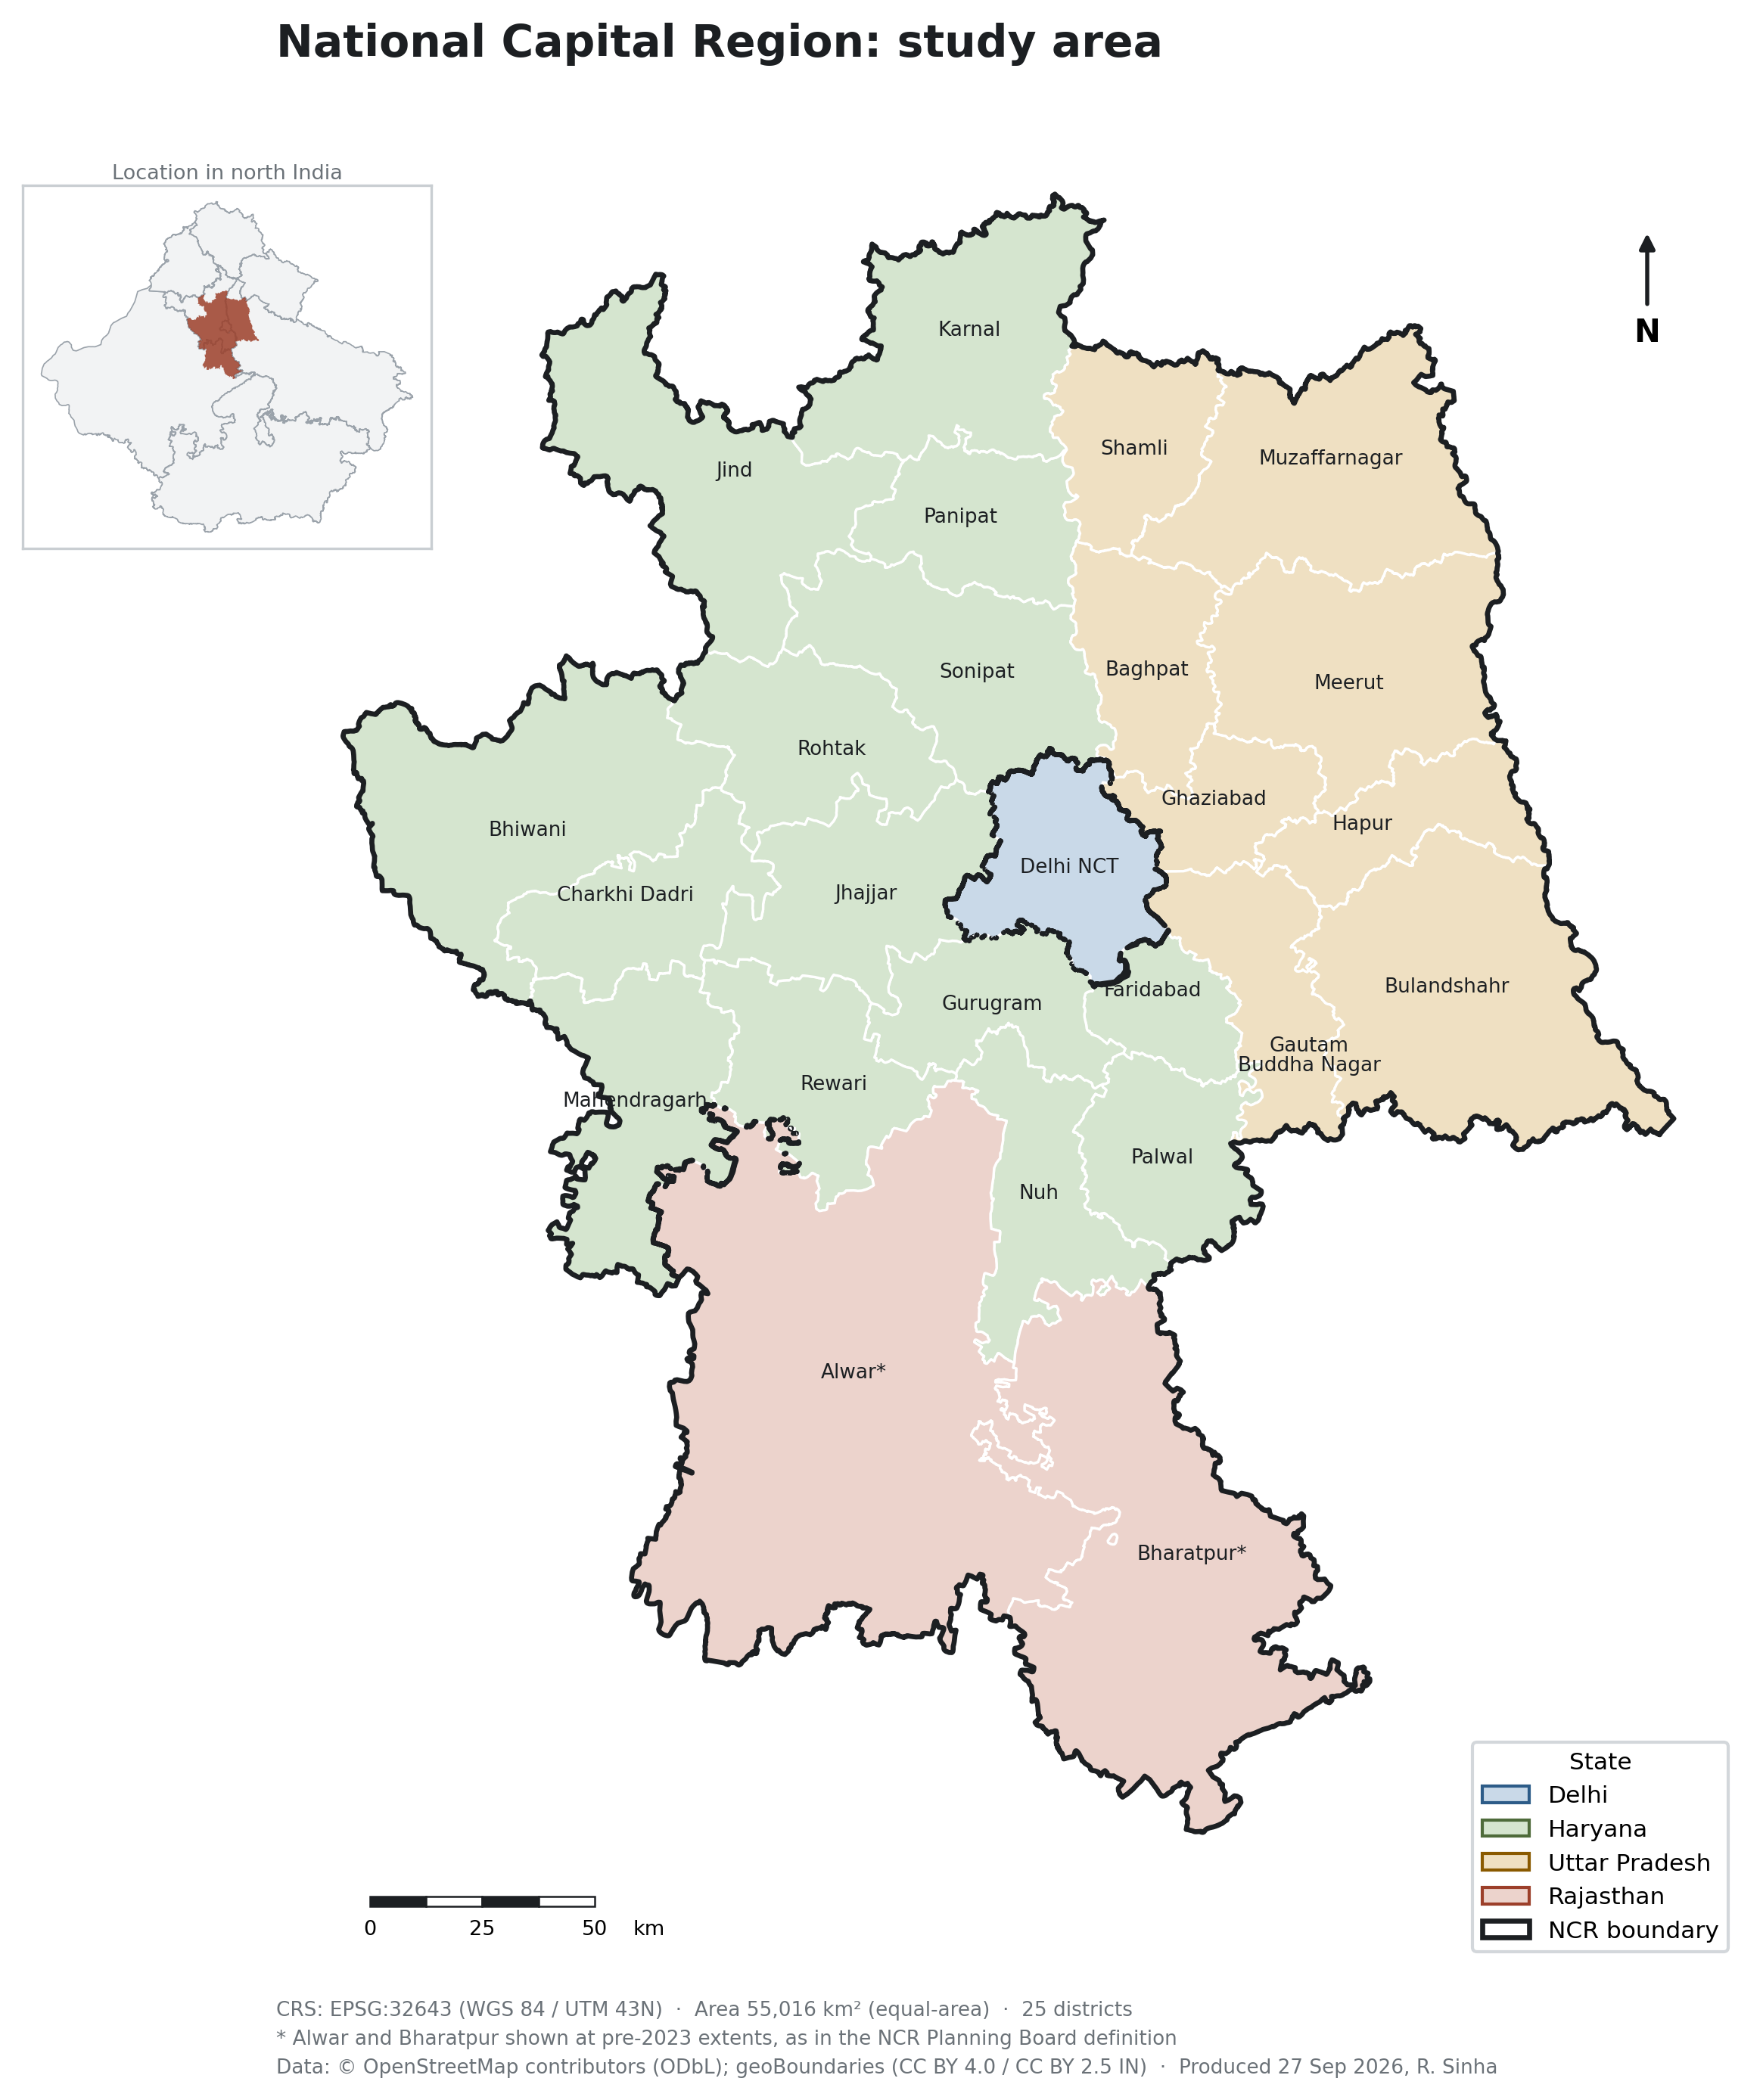
\includegraphics[width=0.82\textwidth]{../outputs/maps/00_study_area.png}
\caption{Study area. Alwar and Bharatpur at their pre-2023 extents. EPSG:32643.}
\label{fig:area}
\end{figure}

\subsection{Boundary construction and verification}
OpenStreetMap carries Rajasthan's 2023 district reorganisation, in which Alwar
and Bharatpur lost territory to Khairthal-Tijara, Kotputli-Behror and Deeg. The
NCR is defined on the pre-2023 districts, so they were rebuilt:
old Bharatpur = Bharatpur + Deeg; old Alwar = Alwar + Khairthal-Tijara + the part
of Kotputli-Behror inside the geoBoundaries ADM2 Alwar polygon. geoBoundaries was
rejected for Delhi in an earlier project because its delineation predates 2012;
that same property makes it correct here. Slivers under 5~km$^2$ from the coarser
geoBoundaries line were dropped.

\begin{table}[H]
\centering\small
\begin{tabular}{@{}lrrr@{}}
\toprule
Unit & This study (km$^2$) & Reference (km$^2$) & Deviation \\
\midrule
NCR total              & 55{,}016 & 55{,}083 (NCRPB)       & $-0.12$\% \\
Alwar, pre-2023        &  8{,}355 &  8{,}380 (Census 2011) & $-0.30$\% \\
Bharatpur, pre-2023    &  5{,}059 &  5{,}066 (Census 2011) & $-0.14$\% \\
\bottomrule
\end{tabular}
\caption{Boundary verification. Areas in an India-centred Albers equal-area
projection. Reference figures checked 13 October 2026 against the NCRPB
constituent-area table (55{,}083~km$^2$) and Census 2011 district areas. The two
Rajasthan figures sum to 13{,}446~km$^2$, which agrees with the NCRPB Rajasthan
sub-region (13{,}447~km$^2$).}
\end{table}

Without the reconstruction, about 3{,}200~km$^2$ of Rajasthan would have been
omitted from the study area.

% ------------------------------------------------------------ 4
\section{Data sources}

{\small
\begin{longtable}{@{}P{2.9cm} P{3.5cm} P{2.1cm} P{3.1cm} P{1.8cm}@{}}
\toprule
Dataset & Provider / access & Licence & Use & Status \\
\midrule
\endhead
District boundaries & OpenStreetMap, via Overpass API & ODbL & Haryana, UP, Rajasthan districts & Fetched \\
Delhi NCT boundary & OpenStreetMap, from earlier Delhi project & ODbL & Delhi portion of NCR & Verified \\
geoBoundaries IND ADM2 & William \& Mary geoLab & CC BY 4.0 & Cut Kotputli-Behror to pre-2023 Alwar & Used \\
geoBoundaries IND ADM1 (simplified) & William \& Mary geoLab; source DataMeet / ECI & CC BY 2.5 IN & Locator inset only & Used \\
SentinelKilnDB & IIT Gandhinagar Sustainability Lab, Hugging Face & CC BY-NC 4.0 & Training and testing the detector & Used \\
Authors' code & GitHub \texttt{rishabh-mondal/ NeurIPS\_2025} & Not stated & Read to match image processing & Read \\
Sentinel-2 L2A (harmonised) & Copernicus / ESA, via Google Earth Engine & Copernicus free licence & Median composites for detection; per-scene SWIR for firing & Used \\
ESA WorldCover 2021 (10 m) & ESA, via Google Earth Engine & CC BY 4.0 & Land-cover filter; school built-up check & Used \\
School locations & NIC SchoolGIS, via \texttt{datameet/ udise\_schools} & Not stated & School points (33{,}648 after location and shared-point checks) & Used, checked \\
School enrolment & UDISE+ (Ministry of Education) & GODL-India (open tables) & Children per school & Not used: access refused (HTTP 403) \\
WorldPop 2020 age--sex (100 m) & WorldPop, University of Southampton, via Earth Engine & CC BY 4.0 & Children aged 5--14 & Used (modelled) \\
OpenStreetMap features & OSM contributors, via Overpass API & ODbL & Non-kiln heat sources (airports, power plants, works) & Used \\
Google Earth historical imagery & Google / Maxar, Airbus & Viewing only & Visual audit of 25 kilns & Used (viewed, not redistributed) \\
GRAP orders and schedules & CAQM document index (89 orders, Oct 2022 -- May 2026; schedules of 13 Dec 2024 and 21 Nov 2025) & Government publication & Which activities close at each stage & Read \\
Siting rules & CPCB notification (2022) & Government publication & 800~m / 1~km / 500~m rules & Read \\
Kiln emission factors & World Bank (2020), Table 2.1 (from Weyant et al.\ 2014 and others) & CC BY 3.0 IGO & PM$_{2.5}$ and BC per kg of brick & Used \\
Reference areas & NCR Planning Board; Census of India 2011 & --- & Boundary verification & Verified \\
\bottomrule
\end{longtable}
}

% ------------------------------------------------------------ 5
\section{Methodology}

\subsection{Training data}
SentinelKilnDB contains 114{,}300 Sentinel-2 patches (128$\times$128~px at 10~m)
with 97{,}648 oriented boxes in three classes: CFCBK (0), FCBK (1), Zigzag (2).
Image names give the patch centre as \texttt{lat\_lon}. 4{,}076 patches with
5{,}954 boxes fall inside the NCR; the count includes duplicates from the 30~px
patch overlap.

Two properties of the dataset shape the design:
\begin{enumerate}[leftmargin=*]
\item \textbf{It is not wall-to-wall inside the NCR.} Every NCR patch contains a
kiln, so the dataset cannot serve as a complete census. The detector must be run
over the full area.
\item \textbf{Documentation and code disagree on dates.} The README states
November 2023 -- February 2024; the download script filters 1 January 2024 --
28 February 2025. This does not affect the change analysis, because both seasons
are mapped by the same detector on imagery whose dates this study controls.
\end{enumerate}

\subsection{Image processing}
Matched to the dataset authors' code: Sentinel-2 surface reflectance bands B4,
B3, B2; QA60 cloud mask; patches of 128~px with 30~px overlap; each band of each
patch stretched independently to 0--255 by its own minimum and maximum.

\subsection{Spatially separated training and test sets}
All 4{,}076 NCR patches form the test set; the detector sees no NCR imagery in
training. Training and validation patches come from a 150~km ring around the NCR,
split 80/20 by 0.5° spatial blocks. A 2~km strip outside the NCR boundary is
excluded, since 1.28~km patches overlap and a border kiln could otherwise appear
on both sides. Kiln-free patches (25\% of the positive count) are drawn from
outside the NCR so the detector learns background.

\begin{table}[H]
\centering\small
\begin{tabular}{@{}lrrr@{}}
\toprule
Set & Patches & With kilns & Kiln boxes \\
\midrule
Train (ring)      & 9{,}029 & 7{,}147 & 9{,}573 \\
Validation (ring) & 2{,}657 & 2{,}202 & 2{,}727 \\
Test (NCR)        & 4{,}076 & 4{,}076 & 5{,}954 \\
\bottomrule
\end{tabular}
\caption{Training split. Box counts include duplicates from patch overlap.}
\end{table}

\textbf{Leakage in the benchmark's own split.} SentinelKilnDB splits patches
randomly by class. Because patches overlap by 30~px, a test patch can share
ground with a training patch. Measured with a Chebyshev-distance test on patch
centres, \textbf{76.6\% of the benchmark's test patches overlap at least one
training patch}. Published scores on that split are therefore likely to be
optimistic; the spatially held-out NCR test used here is stricter, and lower
scores should be expected.

\subsection{NCR imagery}
The NCR is covered by 630 tiles of 1{,}024 $\times$ 1{,}024~px (10.24~km) on a
10~m grid in EPSG:32643, each requested with an explicit pixel transform so
that a kiln falls on the same pixel in both seasons. Each season is the
per-pixel median of Sentinel-2 surface-reflectance scenes with under 20\% cloud,
QA60 opaque and cirrus pixels masked, over identical months
(1 Nov -- 1 Mar) in 2023--24 and 2025--26.

\textbf{Domain check.} Six dataset patches were compared with the same ground cut
from this study's 2023--24 composite. Geometry agrees exactly. Radiometry does
not: the dataset's single-scene patches show bare or yellow fields where the
seasonal median shows green winter crops (median pixel correlation 0.60).
Kilns look alike in both; the background differs. The cost of this shift is
measured directly in Section~\ref{sec:accuracy}. It cost 0.14 F1. Retraining on
patches cut from this study's own composite was tried and rejected (see
\emph{Rejected method}). The shortfall was handled instead by the land-cover
and firing checks.

\subsection{Reference kiln points}
Dataset boxes inside the NCR were converted to ground positions from each patch
centre and box offset, and boxes of the same class within 60~m were merged.
5{,}954 boxes reduce to \textbf{4{,}114 kilns} (3{,}706 Zigzag, 382 FCBK,
26 CFCBK). One kiln appears in up to eight patches: a quarter of NCR patch
centres have a neighbour only $\sim$350~m away rather than the nominal 980~m
stride, consistent with the dataset being built from overlapping state-wise
tile runs. The merge removes these duplicates.

\subsection{Children resident near kilns}
School-level enrolment requires registered UDISE+ access, and the open
block-level tables on data.gov.in refused automated access (HTTP 403). As a
second, independent exposure measure, resident children aged 5--14 are taken
from WorldPop 2020 age--sex structured population (100~m). This is a modelled
estimate and is reported as such.

\subsection{Change between seasons}
Change is measured by firing at fixed locations, not by re-detection, so the
detector's misses cannot pose as closures. Each 2023--24 firing-verified kiln is
re-tested in the 2025--26 season (1 November 2025 -- 1 June 2026) at the same
place: \emph{continuing} if hot frequency is still $\geq$ 0.12, otherwise
\emph{stopped}. A 2025--26 detection is \emph{new} if it fires in 2025--26, has
no 2023--24 detection within 60~m and did not fire there in 2023--24
(\texttt{analysis/kiln\_change.py}).

% ------------------------------------------------------------ 6
\section{Results}

\subsection{Wall-to-wall NCR scan}
The ring detector (confidence 0.25) was run over all 630 tiles for each season:
128~px patches, 30~px overlap, per-patch stretch, detections within 50~m merged.
It returned 14{,}395 kilns in 2023--24 and 13{,}499 in 2025--26 --- 3.5 times the
4{,}114 reference kilns --- with 81\% labelled FCBK against 90\% Zigzag in the
reference. Neither figure was accepted without diagnosis.

\textbf{Diagnosis.} Inside reference-covered patches the detector recovers 65\%
of reference kilns and 67\% of its detections match one, consistent with the
held-out test. 73\% of detections lie outside reference coverage, where the
reference cannot judge them. Land cover separates the two groups (WorldCover
2021, sample of 3{,}000): matched detections sit on bare (68\%) or grass/open
(26\%) ground, the brick yard; unmatched detections mostly on cropland (48\%),
trees and shrub (11\%) and built-up land (9\%).

\textbf{Land-cover filter.} A detection is kept if at least 40\% of the
WorldCover pixels within 40~m are bare or grass/open. The threshold was chosen
as the F1 maximum on reference-covered detections; F1 is flat (0.69) from 0.05
to 0.50, so the choice is not sensitive. There, precision rises from 0.67 to
0.74 for a recall loss of 0.68 to 0.65. Across the NCR the filter removes 57\%
of detections: \textbf{6{,}140 kilns in 2023--24 and 5{,}758 in 2025--26}.
Kilns built on cropland after 2021 may be wrongly dropped.

\textbf{Verification by firing.} A blind visual review of 60 detections was
attempted and abandoned: at basemap resolution a non-specialist reviewer could
not reliably tell kilns from brick-coloured fields, so that review would have
measured the reviewer, not the map. Detections were instead verified with the
hot-spot signal validated above, which needs no interpretation. For each point,
hot frequency is the share of clear Sentinel-2 scenes (1 November 2023 --
1 June 2024) with NHI$_{SWIR} > 0$, maximum within 40~m.

\begin{figure}[H]
\centering
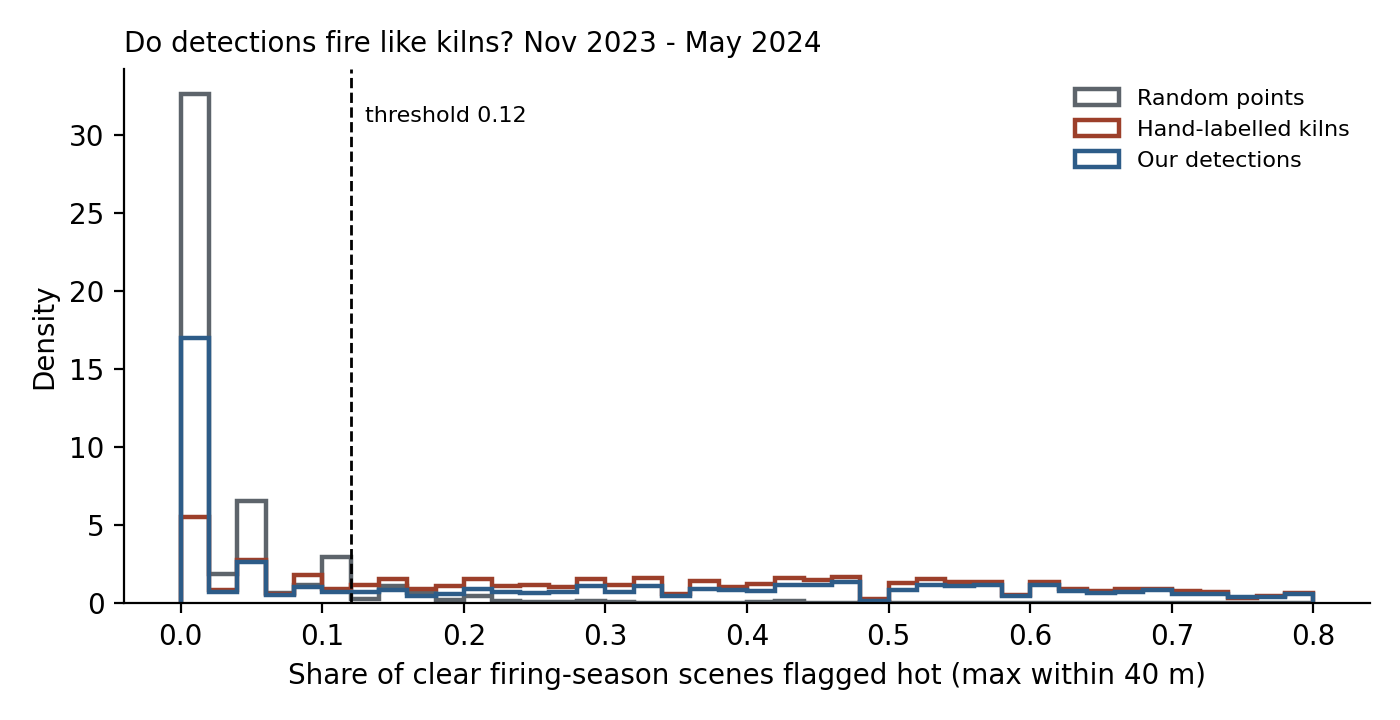
\includegraphics[width=0.85\textwidth]{../outputs/figures/06_firing_verify.png}
\caption{Hot frequency at hand-labelled kilns, random points and detections.}
\end{figure}

The threshold separating kilns from random points was taken from the data
(maximum of Youden's $J$): hot frequency $\geq$ 0.12, met by 75.6\% of the
4{,}114 reference kilns and 8.4\% of 1{,}000 random points. 56.1\% of filtered
detections meet it. If a fraction $p$ of detections are kilns,
$56.1 = 75.6p + 8.4(1-p)$, giving an \textbf{implied precision of 0.71}. This
agrees with the 0.74 measured directly against the reference inside covered
patches, from an entirely independent signal. As a further independent check,
78\% of the 179 kilns tagged \texttt{man\_made=kiln} in OpenStreetMap lie within
100~m of a filtered detection.

\textbf{Two kiln layers are carried forward.}
\begin{itemize}[leftmargin=*]
\item \emph{All filtered detections} (6{,}140): precision $\approx$ 0.71--0.74,
recall $\approx$ 0.65--0.78.
\item \emph{Firing-verified kilns} (3{,}447, hot frequency $\geq$ 0.12):
estimated precision 0.96, since only 8.4\% of non-kilns pass the firing test.
Kilns idle in 2023--24 are excluded, so this layer is a lower bound on active
kilns.
\end{itemize}
Headline exposure figures use the firing-verified layer and are stated as
``at least''. The idle-kiln exclusion makes the precision estimates conservative.

\textbf{Kiln type is not reliable on this imagery.} The FCBK/Zigzag split
disagrees with the reference by a wide margin, so kiln type is not used in any
result until it can be validated.

\subsection{Open question: not everything that burns is a kiln}
\textbf{How it arose.} Reviewing the firing-verified layer in QGIS, the analyst
found a ``kiln'' on the apron of Indira Gandhi International Airport, Delhi. It
passed both checks: the detector saw a small bright rectangle on ground that
WorldCover classes as bare, and the firing test saw heat. The firing test asks
only \emph{is something hot in shortwave infrared?}; jet exhaust, sun-heated
pavement, furnaces, flares and boilers can all answer yes. Firing confirms
\emph{a heat source}, not \emph{a kiln}.

\textbf{How large is the problem?} Firing-verified points were overlaid on
OpenStreetMap aerodromes, power plants and industrial land (Overpass API,
2{,}249 polygons; \texttt{analysis/heat\_source\_check.py}). 165 of 3{,}447 fall
inside such a polygon, but most of those polygons are small (median 1.4~ha,
91\% under 10~ha) and unnamed --- brick fields that mappers drew as industrial
land, i.e.\ real kilns. Counting only points inside a named non-kiln facility,
an industrial estate of 10~ha or more, or an airport leaves \textbf{17 likely
non-kiln heat sources} (15 outside Delhi, 0.4\% of the layer): Panipat Refinery,
Noida International Airport (under construction), large industrial estates in
Gautam Buddha Nagar, Meerut, Hapur, Rewari, Alwar and Gurugram, and two Delhi
bus depots.

\textbf{Status: plausible but unconfirmed, and a lower bound.} OpenStreetMap is
incomplete --- IGI itself was not caught, because the airport is mapped as a
multipolygon relation, which the query did not request. The effect on the
headline is small (removing the 15 would change the lower estimate by under
0.5\% of kilns), but the principle matters: \emph{a thermal signal needs a
context check}.

\textbf{Rectification method.} Two independent checks are
applied to every firing-verified point, and the headline is reported both
before and after the exclusion (\texttt{analysis/nonkiln\_flag.py}).
\begin{enumerate}[leftmargin=*]
\item \emph{Seasonality (a physics check).} Brick kilns shut down in the monsoon
(July--September); the go/no-go test found them hot in only 2\% of monsoon
scenes. Refineries, steel furnaces, power plants and sun-heated airport pavement
stay hot all year. A point that is still hot in the monsoon is therefore
probably not a kiln. Monsoon hot frequency is measured over July--September 2024
and 2025 (scene cloud $<$ 60\%, clouds masked per pixel), and the cut-off is set
from the distribution at the 4{,}114 reference kilns, not assumed
(\texttt{analysis/monsoon\_heat.py}).
\item \emph{Location (a context check).} Points are dropped if they fall inside
an airport, power plant, refinery or other works, or a large industrial estate,
using OpenStreetMap features mapped either as ways \emph{or as multipolygon
relations} --- the form in which IGI Airport is mapped and which the first
version of the check missed (\texttt{analysis/heat\_source\_check.py}).
Small unnamed industrial polygons ($<$ 10~ha) are kept: they are brick fields
mapped as industrial land, and behave like kilns (2\% monsoon-hot).
\end{enumerate}

\textbf{Result.}
\begin{itemize}[leftmargin=*]
\item \emph{Cut-off from the data.} Monsoon hot frequency at the reference kilns
has median 0.00 and 99th percentile \textbf{0.30}; that percentile is the
cut-off, so about 1\% of real kilns are sacrificed. Monsoon values are noisier
than the go/no-go 2\% suggests because few monsoon scenes are clear, which is
why a high percentile rather than a small value is used.
\item \emph{The two checks agree.} 48\% of location-flagged points are
monsoon-hot, against 4\% of all other points --- an independent confirmation
that the location check finds non-kilns.
\item \emph{They also catch different things.} The IGI apron point has a monsoon
hot frequency of 0.00 (jet exhaust is intermittent, not continuous) and is caught
only by location; most monsoon-hot points lie in facilities OSM does not map.
\item \emph{Removed: 157 of 3{,}447 points} (location only 12, monsoon only 134,
both 11), \textbf{leaving 3{,}290 kilns}. About 38 of the removals are expected
to be real kilns (1.09\% of the layer). Before removal about 4\% of the layer
($\approx$ 148 points) were estimated to be non-kilns; removing $\approx$ 119
of them raises the estimated precision from 0.96 to about 0.99 (\emph{superseded:
the visual audit in Section~\ref{sec:audit} measured 0.91}; plausible, not
measured).
\item \emph{A further consistency check.} Removed points ``stopped'' between
2023--24 and 2025--26 only 5.7\% of the time, against 13.8\% for the kept
kilns: year-round heat sources keep burning, as non-kilns should.
\item Removals are spread across industrial districts (Alwar, Karnal 12 each;
Bhiwani, Rewari, Panipat, Sonipat, Hapur 11 each). Half of Delhi's 18 points
(9) are removed by these checks alone.
\end{itemize}
\textbf{Duplicate detections.} Inspecting the web map, the analyst noticed two
kiln points on one kiln. Close pairs (under 120~m) were checked against the
hand-labelled reference: pairs matching a single reference kiln (duplicates) lay
50--68~m apart (17 of 21 under 70~m), while pairs matching two reference kilns
(genuine neighbours) lay 72--118~m apart (3 of 38 under 70~m). Points closer
than 70~m were merged, keeping the one with the highest firing frequency
(\texttt{analysis/dedupe\_kilns.py}): 25 duplicates removed, \textbf{leaving
3{,}265 kilns} (3{,}256 outside Delhi). Because overlapping 800~m zones cover
the same ground, exposure barely changed (605{,}558 to 605{,}292 children;
schools unchanged at 1{,}708); kiln counts and H3 were recomputed. The
emergency-day test (step 23) and the audit sample were drawn before this step,
from the 3{,}290-point layer; at 0.8\% duplicates their conclusions are
unaffected.

The removed points are kept, with the reason, in
\texttt{data/kilns/nonkiln\_removed\_32643.gpkg}. All results below use the
cleaned layer; the values before cleaning are kept in
\texttt{outputs/tables/*\_before\_nonkiln.csv}.

\subsection{Schools and children within 800 m of a kiln}
800~m zones (the CPCB minimum siting distance) were drawn round 2023--24 kilns.
Schools are those passing the location checks and the shared-point check (33{,}648; Section~\ref{sec:fullcheck}). Children are WorldPop
2020 ages 5--14, summed inside the union of zones so overlapping zones count
people once.

\textbf{Delhi excluded.} The 18 firing detections inside Delhi NCT, where
brick kilns are not permitted, sit in the Bawana--Narela industrial belt, near
Old Delhi, on the Yamuna floodplain and on the IGI Airport apron --- more
plausibly industrial furnaces, crematoria and other heat sources than kilns.
None is near a landfill (closest 2.6~km). The non-kiln checks remove 9; the
other 9 are excluded with the rest of Delhi. Including them would add 28{,}127
children and 27 schools to the lower estimate.

\begin{table}[H]
\centering\small
\begin{tabular}{@{}lrr@{}}
\toprule
NCR excluding Delhi NCT & Lower: firing-verified & Upper: all filtered \\
\midrule
Kilns                                  & 3{,}057   & 5{,}715 \\
Kilns with a school within 800~m       & 32.9\%    & 42.6\% \\
Schools within 800~m of a kiln         & 1{,}194   & 3{,}883 \\
Children aged 5--14 within 800~m       & 528{,}161 & 1{,}213{,}026 \\
Share in Uttar Pradesh districts       & 70.9\%    & 60.0\% \\
Share in Haryana districts             & 24.2\%    & 27.4\% \\
Share in Rajasthan districts           &  4.9\%    & 12.6\% \\
Share in the top 3 districts           & 40.9\%    & 33.4\% \\
\midrule
\emph{Before visual check / shared points:} children & 605{,}292 & 1{,}279{,}426 \\
\emph{Before visual check / shared points:} schools  & 1{,}708   & 4{,}542 \\
\emph{Before non-kiln removal:} children & 665{,}738 & 1{,}335{,}400 \\
\emph{Before non-kiln removal:} schools  & 1{,}891   & 4{,}712 \\
\bottomrule
\end{tabular}
\caption{Exposure, 2023--24, after removing non-kiln heat sources, duplicates,
the 208 non-kilns found by the visual checks and the stacked school points
(\texttt{analysis/exposure\_excl\_delhi.py}). The lower estimate is the
headline; every kiln in it that lies within 800~m of a school was checked by eye.}
\end{table}

\textbf{Headline.} About 528{,}000 children aged 5--14 --- 6.4\% of the
NCR's children outside Delhi --- live within 800~m of a firing brick kiln, and
1{,}194 schools stand within that distance (range 528{,}000--586{,}000 children and 1{,}194--1{,}414 schools, see Section~\ref{sec:fullcheck}).
Two-thirds of the exposed children are in the eight Uttar Pradesh districts of
the NCR; the top three by number are Muzaffarnagar, Baghpat and Bulandshahr.
\textbf{By share, Baghpat stands out: 32.3\% of its children --- one in three
--- live within 800~m of a firing kiln}, followed by Shamli (16.3\%) and
Muzaffarnagar (14.7\%) (Figure~\ref{fig:exposuremap}). Removing non-kiln heat
sources cut the estimate by 9\% (60{,}180 children, 183 schools): industrial
sites sit near dense settlement, so each false kiln carried more exposure than a
real one.

\begin{figure}[H]
\centering
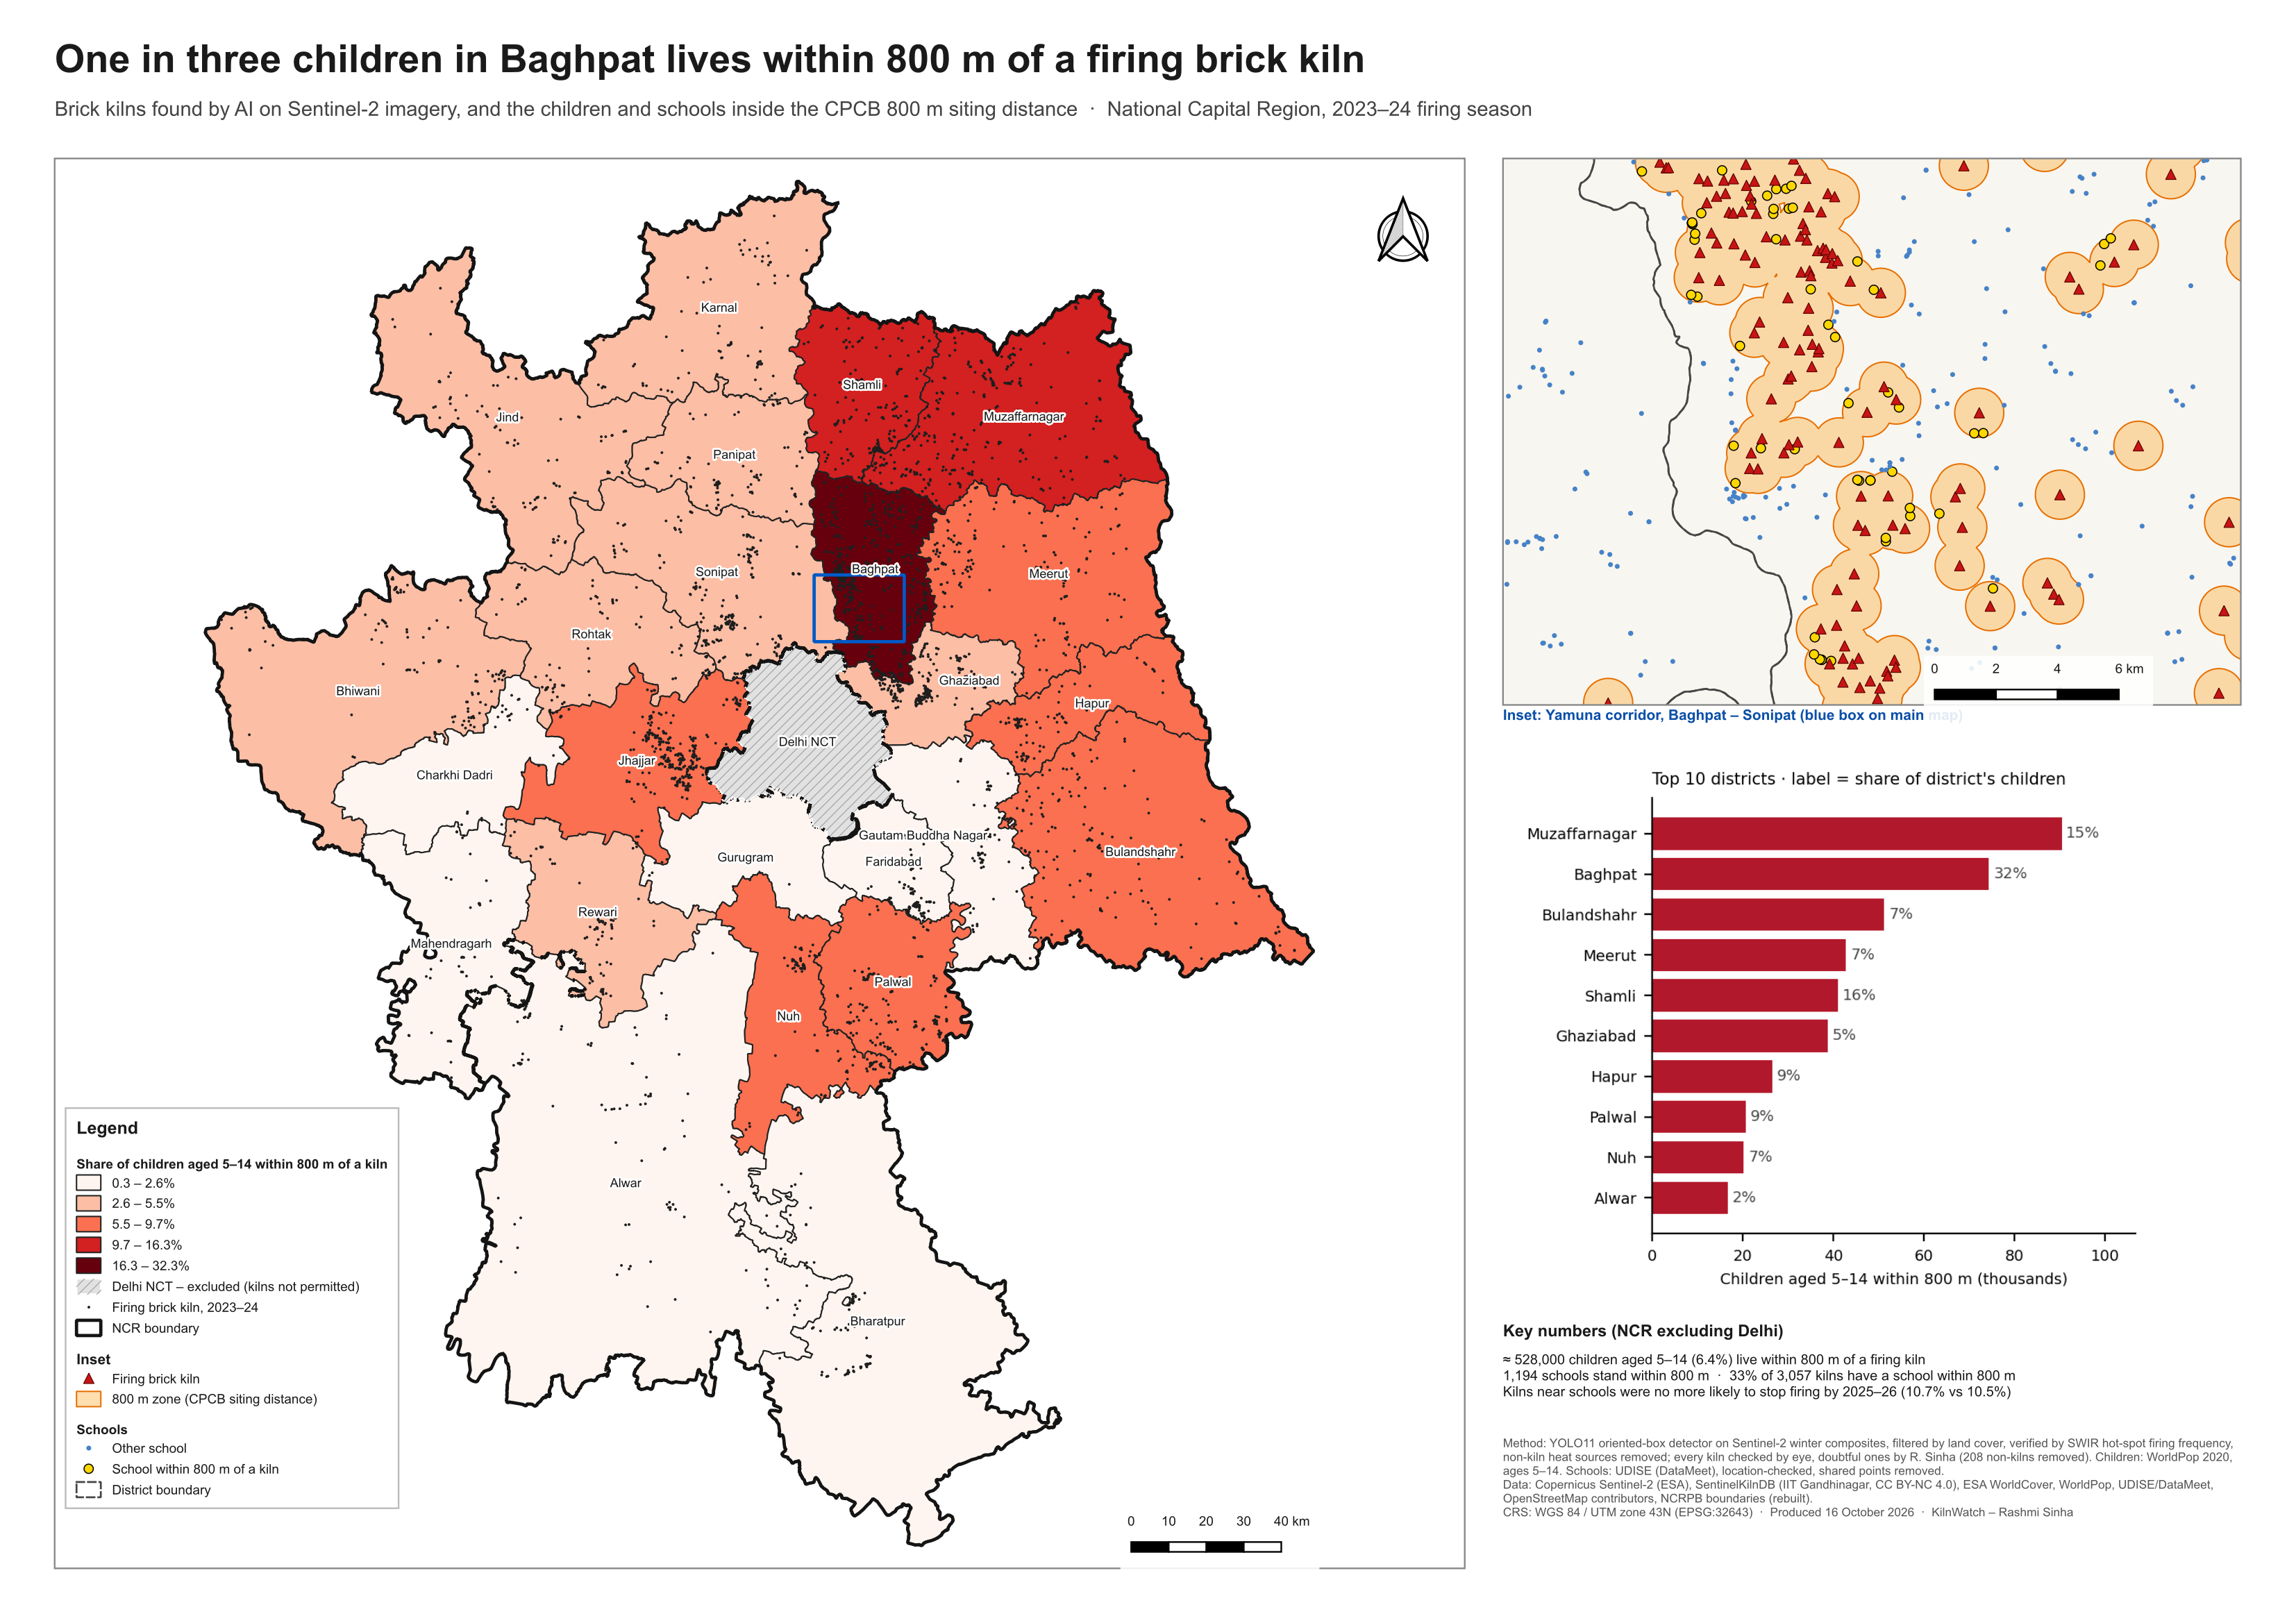
\includegraphics[width=\textwidth]{../outputs/maps/kiln_exposure_map_A3.png}
\caption{Share of children aged 5--14 living within 800~m of a firing brick
kiln, by district, 2023--24 (Jenks classes), with an inset of the Yamuna
corridor and the ten districts with most exposed children. Districts are shaded
by share rather than count, so that population size is not mistaken for
intensity. District child totals: WorldPop 2020 (\texttt{analysis/map\_exposure\_data.py}).
EPSG:32643.}
\label{fig:exposuremap}
\end{figure}

\textbf{Plausibility of WorldPop.} WorldPop 2020 gives the NCR 60.4~million
people, 18.1\% aged 5--14, consistent with the 2011 Census (about 46~million)
plus a decade of rapid growth.

\textbf{H1 --- confirmed.} Predicted $\geq$ 25\% of kilns with a school within
800~m; measured 32.9\% (lower) to 42.5\% (upper).

\textbf{H2 --- rejected as stated.} Predicted that the top three districts hold
more than half the exposed children; they hold 40.9\%. Exposure is regional
rather than concentrated in a few districts: 70\% lies across the eight western
Uttar Pradesh districts of the NCR.

\subsection{Which kilns stopped firing, 2023--24 to 2025--26}
Of 3{,}447 kilns firing in 2023--24, \textbf{2{,}983 were still firing in
2025--26 and 464 (13.5\%) were not}; 71 new firing kilns appeared. After
removing non-kiln heat sources and duplicate detections, 453 of 3{,}265 kilns
(13.9\%) stopped; after the visual checks, 324 of 3{,}057 outside Delhi (10.6\%).

\textbf{Rejected correction.} The plan was to correct the stop rate for the
firing test's miss rate: an active reference kiln fails the test 24.4\% of the
time, so $c = (13.5 - 24.4)/75.6$. That gives a negative rate, which shows the
correction is wrong, not that no kiln stopped. The 24.4\% comes from \emph{all}
reference kilns, including weak and idle ones; the kilns re-tested here were
selected \emph{because} they fired strongly (median hot frequency 0.47, four
times the threshold), so they are far less likely to drop below it by chance.
The miss rate of a selected group cannot be borrowed from the whole population.

\textbf{What can be said.} 13.8\% is an \emph{upper bound} on the stop rate of
real kilns, since some ``stops'' are firing-test misses. An earlier estimate
here assumed the non-kilns would \emph{inflate} the stop rate; the non-kiln
removal showed the opposite (removed points stopped only 5.7\% of the time), so
that assumption is withdrawn. The true stop rate is not yet separable from test
misses; it needs a test--retest estimate of the firing test on strong firers.

\subsection{H3: are kilns near schools closed more often?}
If siting rules were enforced around schools, kilns within 800~m of a school
would stop more often than other kilns. Delhi NCT excluded
(\texttt{analysis/h3\_stop\_near\_schools.py}).

\begin{table}[H]
\centering\small
\begin{tabular}{@{}lrrr@{}}
\toprule
2023--24 firing kilns & Kilns & Stopped by 2025--26 & Stop rate \\
\midrule
School within 800~m    & 1{,}006 & 108 & 10.7\% \\
No school within 800~m & 2{,}051 & 216 & 10.5\% \\
\midrule
Difference & \multicolumn{3}{r}{+0.2 points (95\% CI $-$2.1 to +2.5), $\chi^2$ $p$ = 0.91} \\
\bottomrule
\end{tabular}
\caption{Stop rates by proximity to a school, after both visual checks. With
only near-school kilns checked: 10.8\% vs 13.2\% ($-2.5$, $p$ = 0.06); before any
visual check: 14.6\% vs 13.3\%, +1.3 points ($p$ = 0.31); before non-kiln removal:
14.1\% vs 12.9\% ($p$ = 0.35). The firing test's
error applies equally to both groups, so it shifts both rates, not their
difference.}
\end{table}

\textbf{H3 --- confirmed.} Kilns near schools stop as often as kilns elsewhere
(10.7\% vs 10.5\%; 95\% CI $-2.1$ to $+2.5$ points, so any real difference is
small). The estimate moved twice while the layer was being cleaned, and the moves
are instructive. Before any visual check, near-school kilns looked slightly
\emph{more} likely to stop (+1.3): 60 of the 101 near-school non-kilns were
recorded as ``stopped'' (a stadium does not fire steadily). With only the
near-school group cleaned, they looked \emph{less} likely to stop ($-2.5$,
$p = 0.06$) --- but the far group still held its own false kilns, which also look
like closures. Once the weak-firing kilns away from schools were checked too (65
non-kilns removed), the difference vanished. By state: Haryana 12.7\% near vs
13.1\% far, Uttar Pradesh 10.4\% vs 7.7\%, Rajasthan 6.9\% vs 14.3\% (small
numbers). Two seasons after the baseline, 896 kilns near schools are still firing.

\textbf{Lesson recorded.} Errors in the kiln layer were not random with respect to
the question: false kilns look like closures, and they cluster in towns, near
schools. Cleaning one group only would have produced a borderline ``finding''
($p = 0.06$) that was an artefact; a comparison is only as fair as the checking
of both groups.

\subsection{Can Sentinel-2 see kilns firing? (Phase 3 go/no-go)}
The Normalized Hot-spot Index, NHI$_{SWIR}$ = (B12 $-$ B11)/(B12 + B11)
\cite{marchese2019}, was computed for every clear Sentinel-2 scene of 2024 at
100 known kilns and 100 control points at least 1.5~km from any known kiln
(maximum within 40~m). Hot surfaces emit more at 2.2~$\mu$m than 1.6~$\mu$m;
clay and brick reflect the other way, since clay minerals absorb near 2.2~$\mu$m.

\begin{figure}[H]
\centering
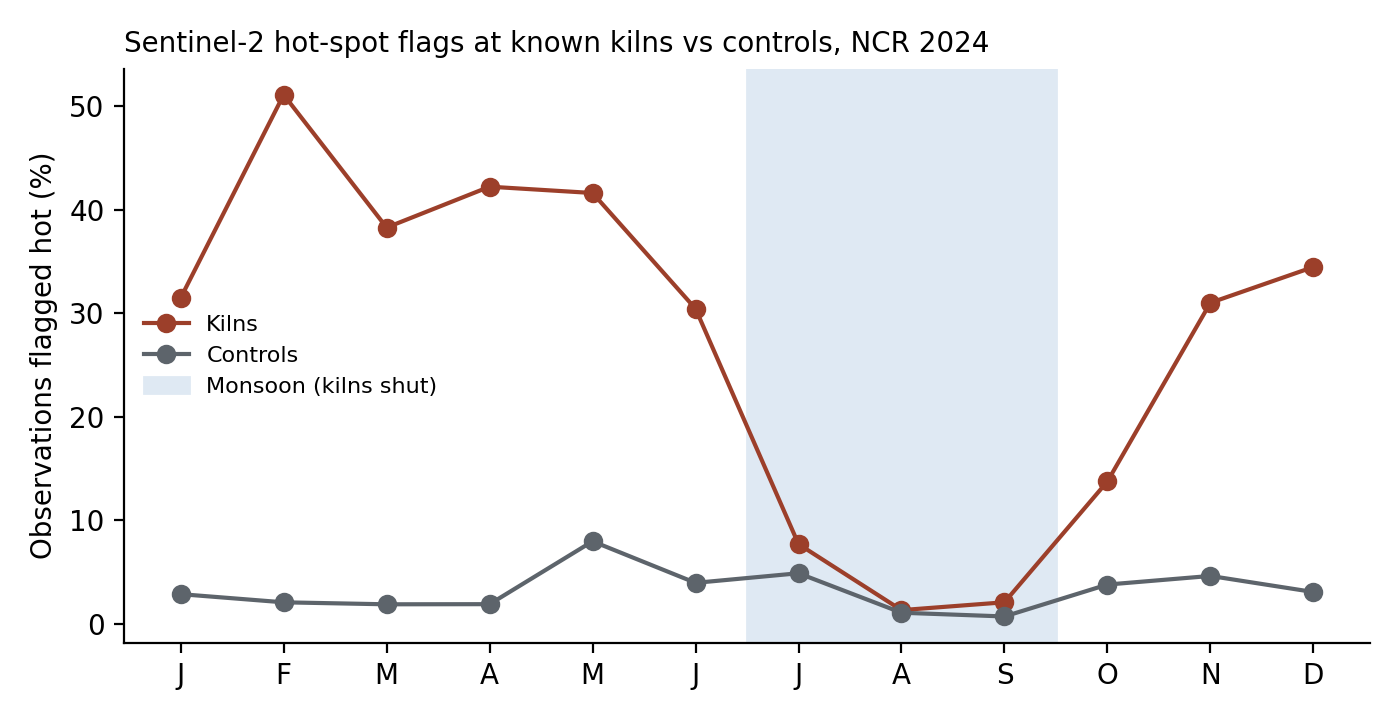
\includegraphics[width=0.85\textwidth]{../outputs/figures/05_firing_test.png}
\caption{Share of clear observations with NHI $>$ 0, by month, 2024.}
\end{figure}

\begin{table}[H]
\centering\small
\begin{tabular}{@{}lrr@{}}
\toprule
 & Dry season (Oct--Jun) & Monsoon (Jul--Sep) \\
\midrule
Kilns (4{,}954 obs.)     & 33.2\% & 2.0\% \\
Controls (6{,}451 obs.)  &  4.0\% & 1.2\% \\
\bottomrule
\end{tabular}
\caption{Observations flagged hot. 90\% of kilns and 51\% of controls were
flagged at least once, so a single flag is not evidence; frequency is.}
\end{table}

\textbf{Confound check.} The monsoon collapse fits kilns shutting, but also wet
ground. A zigzag kiln fires progressively round its trench, so a fire should
move; material should not. For the 30 most frequently flagged kilns the hottest
20~m pixel was located on every flagged date: it occupied a median of 9
distinct pixels, with RMS spread 26~m and maximum displacement 84~m --- the
scale of a kiln loop and well above the $\sim$10~m multi-date registration
error. No kiln's hot spot stayed on one pixel. On its own, a wandering maximum
is not conclusive (a uniformly bright target also yields one), but together
with the sign of the index and the October onset it is strong evidence that
the signal is firing. \textbf{Verdict: go.}

\subsection{GRAP: do brick kilns have to stop?}
All 89 GRAP orders listed by CAQM (October 2022 -- May 2026) were read from the
Commission's document index, and the Stage III/IV invocations and revocations
transcribed with their document identifiers: 40 days with Stage III or IV in
force (three windows) in 2023--24, 44 (six) in 2024--25 and 41 (three) in
2025--26.

\textbf{The GRAP schedules do not close brick kilns.} Both schedules CAQM
publishes (13 December 2024 and 21 November 2025) were read in full. Kilns
appear only under Stage I: pollution rules to be enforced, only approved fuels
to be used, and ``closure in case of violations''. Stage III closes stone
crushers and all mining; the ``brick / masonry works'' it restricts are
construction activities, not kilns. Stage IV adds further restrictions and does
not mention kilns. Press reports that kilns are ``banned at Stage III'' do not
match the current schedules. The 2023--24 season operated under an earlier
schedule no longer listed by CAQM, so kiln coverage then is
\status{unverified}; ban-period analysis is restricted to 13 December 2024
onwards.

The question therefore changes from compliance to policy: during the NCR's
worst air-quality emergencies, stone crushers and mines are shut but kilns are
exempt --- do they keep firing? In the 100-kiln test sample (November--February
2024, before the restriction date and so indicative only) kilns were flagged hot
in 37.3\% of clear observations on Stage III/IV days and 35.2\% on other days;
controls 4.4\% and 2.8\%. Controls also rise on those days, the smoggiest, so
comparisons must be net of controls.

\subsection{The firing calendar, November 2023 -- June 2026 (step 22)}
For every kiln and every calendar month, the share of clear Sentinel-2 scenes
showing heat (NHI$_{SWIR} > 0$, max within 40~m; scene cloud $<$ 60\%, clouds
masked per pixel) was measured, with the number of clear scenes, and the same at
the 1{,}000 random control points (\texttt{analysis/monthly\_firing.py},
\texttt{monthly\_firing\_controls.py}). Months with two or fewer clear scenes
per kiln (January fog, monsoon cloud) are flagged as unreliable.

\begin{figure}[H]
\centering
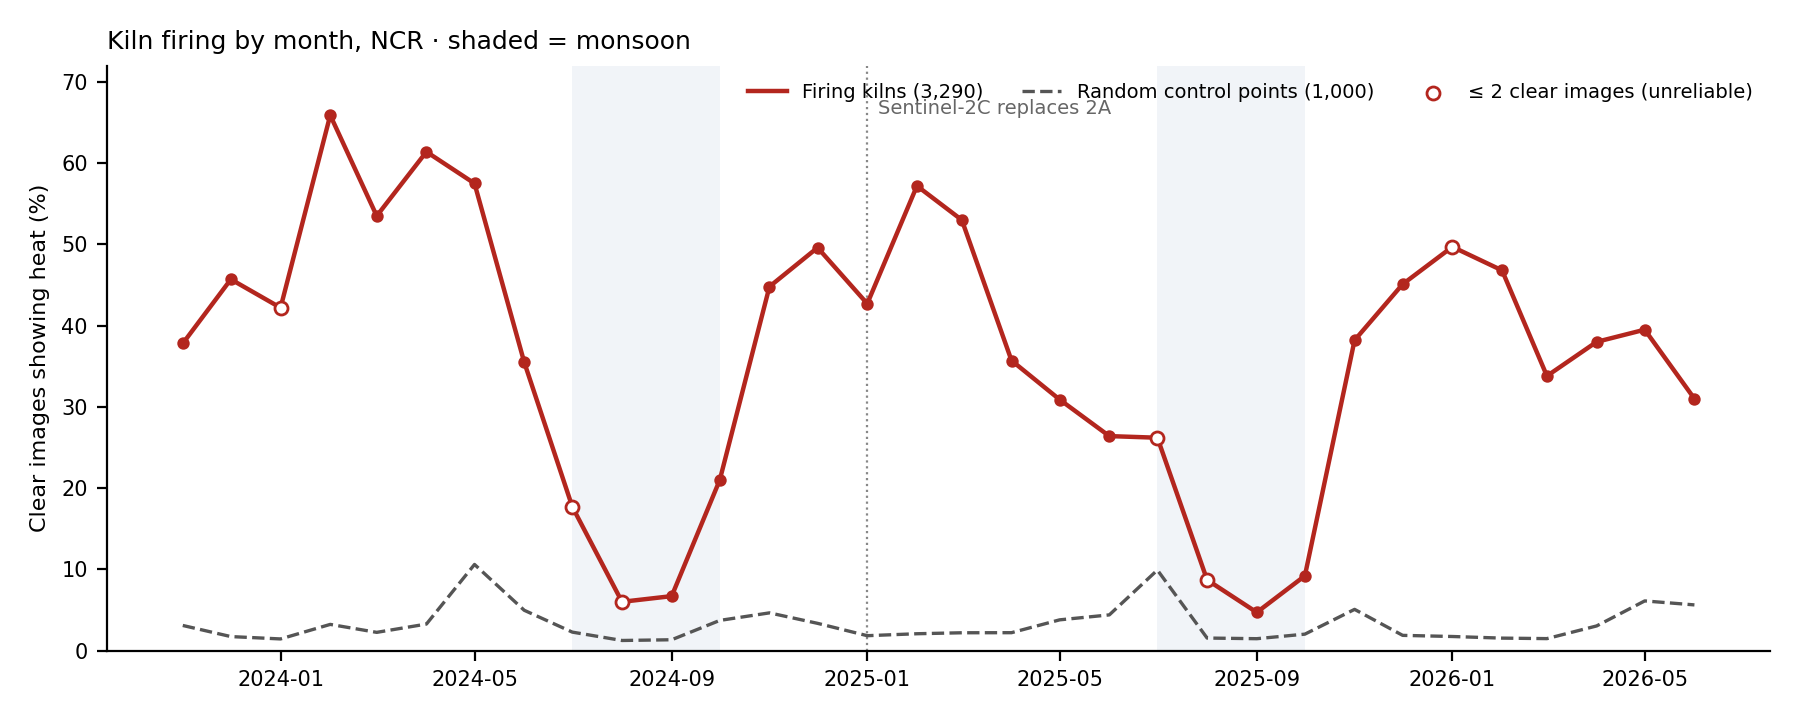
\includegraphics[width=\textwidth]{../outputs/figures/07_monthly_firing.png}
\caption{Share of clear images in which kilns (red) and random points (grey)
show heat, by month. Hollow points rest on two or fewer clear images.}
\end{figure}

\textbf{The season, measured.} Kilns relight in October--November, peak in
February--May (55--66\% of clear images in 2023--24), and drop to near
background in August--September (5--7\% against 1--2\% for controls), matching
the known pattern of monsoon shutdown. This is an independent check that the
heat signal tracks kiln operation.

\textbf{A decline in firing, with an observing-system check.} Dry-season firing
net of the control background fell from 0.50 (2023--24) to 0.42 (2024--25) and
0.37 (2025--26), about a quarter in two seasons. Sentinel-2C replaced
Sentinel-2A in January 2025, so a change in the instrument could mimic a change
on the ground. The control background stayed flat across that date (dry-season
means 4.0\%, 3.0\% and 3.2\%), so the new sensor does not create or suppress
false heat. Controls cannot test sensitivity to real fires, however, so the
decline is \status{plausible, partially checked}: consistent with the 13.9\%
stop rate (step 14) plus lower firing among continuing kilns, but not proven to
be free of a sensor effect.

\subsection{Do kilns keep firing during air-quality emergencies? (step 23)}
\textbf{Design.} 13 December 2024 -- 28 February 2026, November--February only,
3{,}290 cleaned kilns and 1{,}000 random control points. Firing is the share of
clear observations with NHI$_{SWIR} > 0$; the haze effect on smoggy days is
removed by subtracting the controls (difference-in-differences).

\textbf{Rejected first analysis: pseudo-replication.} Treating each kiln as an
independent observation gave kilns hot on 37.0\% of emergency-day scenes against
45.3\% on ordinary days, a net effect of $-8.2$ points with a bootstrap 95\% CI
of $-8.8$ to $-7.6$. Two checks showed this precision was false. (1) Emergency
days cluster in November--January, ordinary days include more February, when
kilns fire more --- a seasonal confound. (2) Re-estimated within each calendar
month, the per-kiln effect swung from $-45$ to $+32$ points between months.
All kilns under one Sentinel-2 pass share that day's atmosphere and viewing
conditions, so the effective sample size is the number of \emph{days}, not
kilns. The per-kiln interval is withdrawn
(\texttt{analysis/grap\_firing.py}, \texttt{grap\_firing\_bymonth.py}, kept as
documented negative results).

\textbf{Corrected analysis: the day as the unit.} For each of 109 days with
imagery, net firing $=$ (share of observed kilns hot) $-$ (share of observed
controls hot). Days observing fewer than 200 kilns were dropped, and only months
containing both emergency and ordinary days were kept, leaving 23 days (10
emergency, 13 ordinary). The emergency effect was estimated within month (month
fixed effects by demeaning), with a bootstrap of days within month for the
interval and a within-month permutation test
(\texttt{analysis/grap\_firing\_daily.py}).

\begin{table}[H]
\centering\small
\begin{tabular}{@{}lr@{}}
\toprule
Net firing on emergency days (mean)             & 42.1 points \\
Net firing on ordinary days (mean)              & 51.7 points \\
Effect of an emergency day, within month         & $-5.5$ points \\
95\% CI (bootstrap of days)                      & $-21.6$ to $+10.0$ \\
Permutation $p$                                  & 0.62 \\
\bottomrule
\end{tabular}
\caption{Kiln firing on GRAP Stage III/IV days, day-level analysis.}
\end{table}

\textbf{Finding.} Kilns clearly \emph{do} fire during the NCR's air-quality
emergencies: on emergency days the share of kilns showing heat exceeded the
background by 42 points on average. This is consistent with the schedules, which
do not require kilns to close. Whether kilns cut back at all could not be
determined: the interval spans a substantial reduction and a small increase.
With a 5-day revisit and frequent cloud and haze on smog days, Sentinel-2 yields
too few usable emergency days (10) to measure a response of plausible size.
This is reported as an \emph{inconclusive} test, not as evidence of no effect;
a geostationary or daily sensor, or kiln-level monitoring, would be needed.

\textbf{Lesson recorded.} The first result looked precise because of a
methodological error, not because the data were informative. Its interval was
about 25 times narrower than the honest one.

\subsection{How much smoke, and how much of it next to schools? (step 24)}
\label{sec:emissions}
\textbf{In one line.} We multiply how many bricks the kilns bake by how much
fine dust each kilogram of brick releases. The result is a range, not a
measurement.

\textbf{Method} (\texttt{analysis/emissions.py}). One season (2023--24), the
3,057 cleaned kilns outside Delhi:
\[
\text{PM}_{2.5}\ (\text{t}) = \text{bricks} \times 3\ \text{kg} \times
\text{EF}\ (\text{g/kg fired brick}) / 10^{6}.
\]
In numbers:
\begin{center}\small
\begin{tabular}{@{}ccccccc@{}}
\toprule
Bricks baked & $\times$ & Weight of a brick & $\times$ & Dust per kg of brick & $=$ & Dust released \\
\midrule
12--18 billion & & 3 kg & & 0.12--0.21 g & & 4,400--11,600 t \\
\bottomrule
\end{tabular}
\end{center}
Low case: $12.2\times10^{9} \times 3 \times 0.12 / 10^{6} = 4{,}400$~t.
High case: $18.3\times10^{9} \times 3 \times 0.21 / 10^{6} = 11{,}600$~t.
\begin{itemize}[leftmargin=*]
\item \emph{Emission factors} come from World Bank (2020) Table~2.1, averaged
from Weyant et al.\ (2014), Greentech (2012) and others~\cite{worldbank2020,weyant2014}.
Zigzag kilns emit 0.12~g PM$_{2.5}$ and 0.035~g BC per kg. Fixed-chimney kilns
emit 0.21 and 0.17. NCR kilns were ordered to convert to zigzag, but the same
report warns the zigzag values ``seem too optimistic'' because most
conversions are not built to standard. Zigzag is therefore the \emph{low} case
and fixed-chimney the \emph{high} case. We cannot tell the two apart at 10~m
(see Future work).
\item \emph{Bricks per kiln per season} are \textbf{assumed}, not measured:
4~million in the low case (CSE's model kiln, 40~lakh a year) and 6~million in
the high case (about 250~billion bricks a year in India divided by about
44,000 kilns gives 5.7~million).
\item \emph{Split between kilns.} Bricks cannot be seen from space, but firing
can. Each kiln's share of the total is proportional to its 2023--24 firing
frequency (\texttt{hot\_frac}), so busy kilns get more. The NCR total does
not depend on this choice; the split between districts and schools does.
\end{itemize}

\textbf{Cross-check.} Weyant et al.'s South Asian totals (0.19~Tg PM$_{2.5}$
from 260~billion bricks) imply 0.73~g per brick. Applied to our 12--18~billion
bricks, that gives 8,900--13,400~t. This falls inside our range, at the upper
end. It shows our numbers are the right order of magnitude, not that they are
correct.

\begin{table}[H]
\centering\small
\begin{tabular}{@{}lrr@{}}
\toprule
 & Low (zigzag) & High (fixed chimney) \\
\midrule
Bricks fired, season & 12.2 bn & 18.3 bn \\
PM$_{2.5}$, all kilns & 4,400 t & 11,600 t \\
Black carbon, all kilns & 1,300 t & 9,400 t \\
PM$_{2.5}$ from kilns with a school within 800 m & 1,300 t & 3,500 t \\
\quad share of total & \multicolumn{2}{c}{30.3\% (32.9\% of kilns)} \\
\bottomrule
\end{tabular}
\caption{Kiln emissions, 2023--24 season, NCR excluding Delhi. Rounded;
the range reflects assumptions, not a statistical interval.}
\label{tab:emissions}
\end{table}

\begin{table}[H]
\centering\small
\begin{tabular}{@{}lrrrr@{}}
\toprule
District & Kilns & Near a school & PM$_{2.5}$ (t, low--high) & of which near schools (low) \\
\midrule
Baghpat & 404 & 159 & 700--1,840 & 269 \\
Muzaffarnagar & 284 & 60 & 440--1,150 & 86 \\
Jhajjar & 286 & 42 & 420--1,090 & 60 \\
Sonipat & 191 & 35 & 360--930 & 64 \\
Ghaziabad & 209 & 79 & 250--660 & 88 \\
Shamli & 141 & 64 & 220--590 & 109 \\
\bottomrule
\end{tabular}
\caption{Top six districts by kiln PM$_{2.5}$
(\texttt{outputs/tables/emissions\_by\_district.csv}).}
\end{table}

\textbf{What it shows.}
\begin{itemize}[leftmargin=*]
\item The NCR's kilns emit roughly \textbf{4,400--11,600~t of PM$_{2.5}$} in
a season. About \textbf{30\%} comes from kilns within 800~m of a school.
\item Kilns near schools fire slightly \emph{less} often than average: 32.9\% of
kilns produce 30.3\% of emissions.
\item \textbf{Baghpat} again stands out. It emits the most of any district,
and 38\% of its kiln emissions (270 of 700~t, low case) come from kilns near
schools.
\item Most exposed schools have \textbf{one} kiln within 800~m. The worst
case, JHS Rampur Kheri in Shamli, has \textbf{12}, emitting about 25~t of
PM$_{2.5}$ a season in the low case. Rampur Kheri, Matiyala (Ghaziabad, 10)
and Biharipur (Baghpat, 7) are where on-site air monitoring would tell the
most (\texttt{outputs/tables/emissions\_top\_schools.csv}).
\end{itemize}

\begin{figure}[H]
\centering
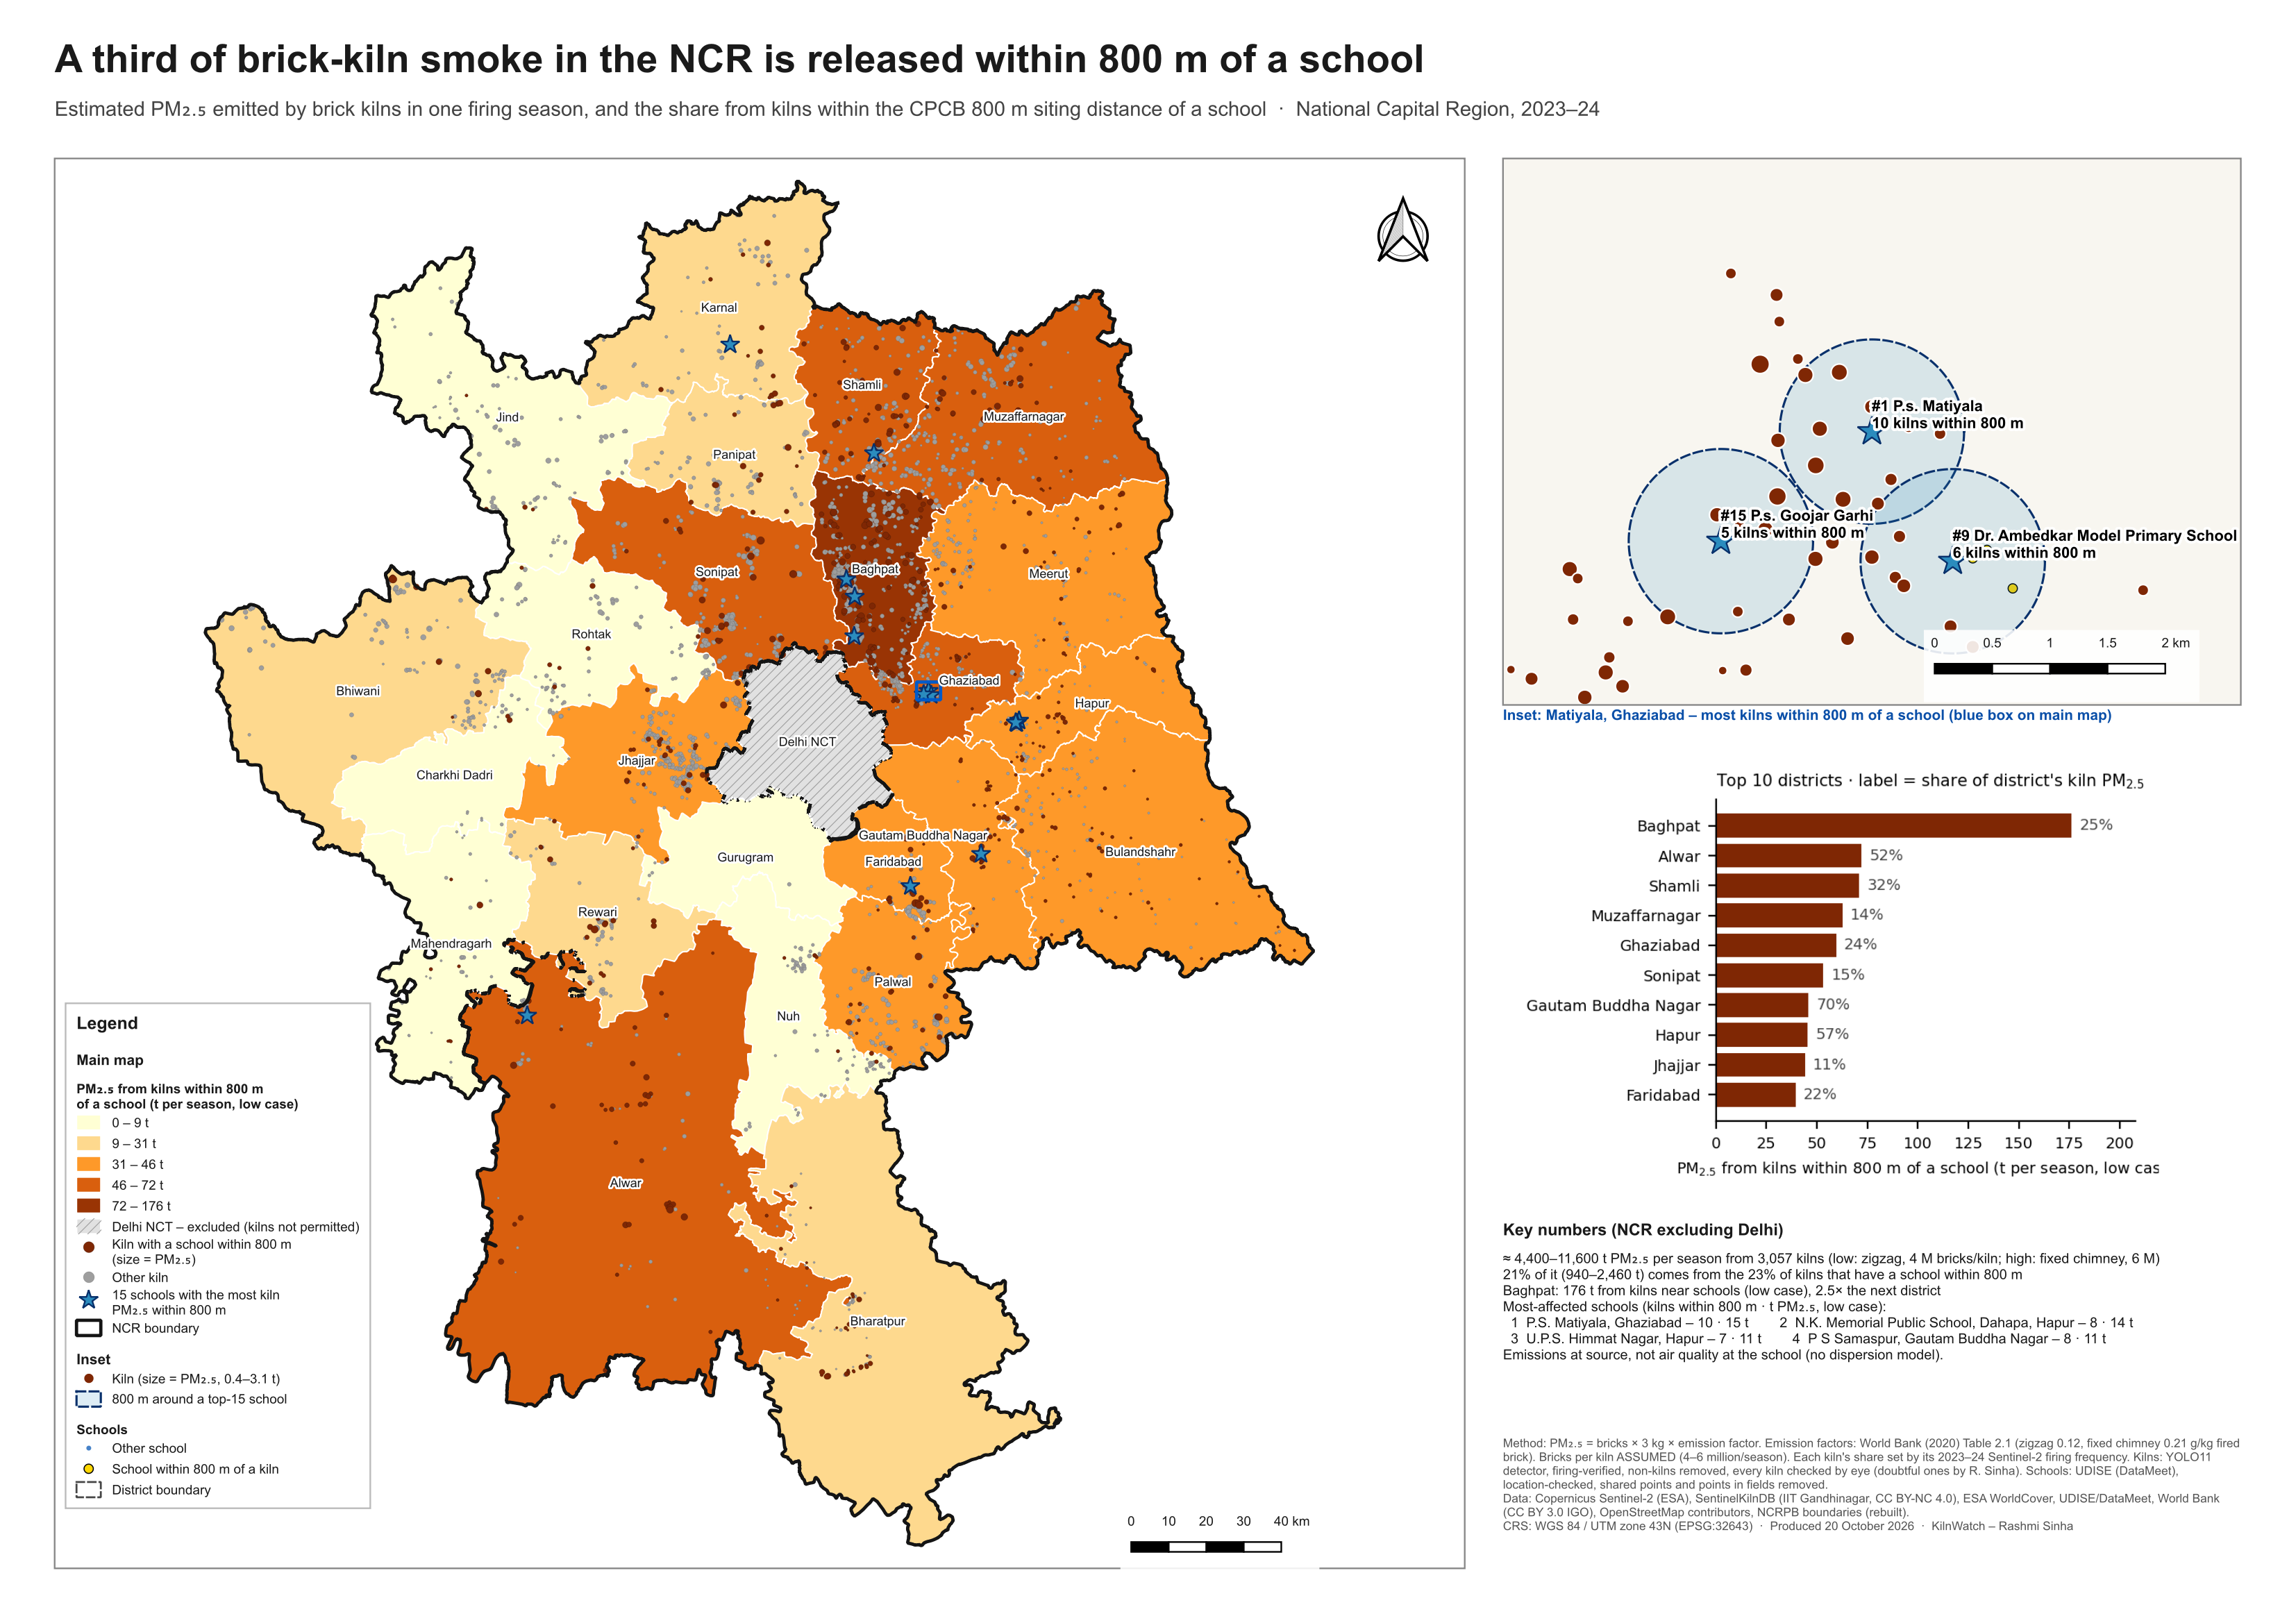
\includegraphics[width=\textwidth]{../outputs/maps/kiln_emissions_map_A3.png}
\caption{Finished map (step 26): PM$_{2.5}$ from kilns within 800~m of a school,
by district (tonnes per season, low case, Jenks classes). Kilns are sized by
estimated PM$_{2.5}$. Stars mark the 15 most-affected schools. The inset shows
Rampur Kheri, Shamli, where 12 kilns lie within 800~m of one school. Districts
are shaded by tonnes rather than tonnes per km$^2$: these are emissions at
source, and dividing by area would imply a spread of smoke that has not been
modelled. Large districts with scattered kilns (Alwar) therefore rank higher
than a density map would put them. A3 PDF:
\texttt{outputs/maps/kiln\_emissions\_map\_A3.pdf}; QGIS layout ``Emissions map
A3''.}
\label{fig:emissionsmap}
\end{figure}

\textbf{What it does not show.} Emissions are not exposure. Where the smoke
goes depends on wind, stack height and mixing depth, which would need a
dispersion model (e.g.\ AERMOD). The table ranks \emph{sources} near schools,
not concentrations inside them. Labels: emission factors are
\emph{published, measured on few kilns}; bricks per kiln is \emph{assumed};
the firing-frequency split is \emph{measured}.

\subsection{Rejected method: fine-tuning on this study's imagery}
To remove the domain shift, the ring training patches were re-fetched from this
study's 2023--24 median and the detector fine-tuned for five epochs from the
best ring model. It made matters worse at every confidence threshold
(point-match F1 on this study's imagery, 617 NCR patches):

\begin{table}[H]
\centering\small
\begin{tabular}{@{}lrrrrrr@{}}
\toprule
Confidence threshold & 0.05 & 0.10 & 0.15 & 0.25 & 0.35 & 0.50 \\
\midrule
Ring model (kept)  & 0.58 & 0.61 & 0.63 & \textbf{0.64} & 0.62 & 0.48 \\
Fine-tuned         & 0.42 & 0.53 & 0.54 & 0.35 & 0.14 & 0.01 \\
\bottomrule
\end{tabular}
\end{table}

The likely cause is label noise: dataset labels come from single scenes as late
as February 2025, so kilns built after the 2023--24 composite are labelled where
the image shows none, teaching the model to under-predict. The fine-tune is
retained in the code (\texttt{finetune\_detector.py}) as a documented negative
result. The ring model at confidence 0.25 is used throughout.

The share of Zigzag kilns among NCR patches in the training data (3{,}669 of
4{,}234 class occurrences, 87\%) is consistent with the directive that kilns in
the NCR convert to zigzag technology. This is a plausibility check on the labels,
not a finding.

% ------------------------------------------------------------ 7
\section{Accuracy assessment}\label{sec:accuracy}


\subsection{School location accuracy}
Of 43{,}904 NCR school points, 10.5\% sit 9--57~km (median) from the district
named in their own record and are excluded. Among the rest, a visual check of 30
random points against high-resolution imagery found 14 on a building and 16 on
open land (53\%, 95\% CI roughly 36--70\%). Schools often look like the houses
around them, so the check asked only the objective question: building or open
land.

The same question was automated for every school as the distance to the
nearest ESA WorldCover 2021 built-up pixel. All 14 visual ``building'' points
are within 50~m of built-up land; 10 of the 16 ``open land'' points are too ---
the point sits on a field or yard beside its village. Agreement 67\%.

\begin{table}[H]
\centering\small
\begin{tabular}{@{}lrr@{}}
\toprule
Distance to nearest built-up & Schools & Share \\
\midrule
On built-up & 24{,}371 & 62.0\% \\
1--50 m     &  7{,}476 & 19.0\% \\
51--100 m   &  1{,}825 &  4.6\% \\
101--300 m  &  3{,}066 &  7.8\% \\
301--800 m  &  2{,}136 &  5.4\% \\
$>$ 800 m   &    403   &  1.0\% \\
\bottomrule
\end{tabular}
\caption{A lower bound on location error, since a school is always a building.}
\end{table}

Most points are displaced by less than 300~m, small against an 800~m rule.
Schools more than 300~m from any built-up land (6.4\%) are treated as
unreliable and excluded from the main count; results are reported with and
without them.

\textbf{How much do position errors move the school count?} The analyst noticed
that many school points do not fall on a school in Google Maps. Rather than
re-locate 33{,}648 schools by hand, every point was moved in a random direction
by a random distance (Rayleigh-distributed, i.e.\ the radial error of a 2-D normal)
and the schools within 800~m of a kiln recounted, 500 times per scenario
(\texttt{analysis/school\_position\_sensitivity.py}).

\begin{table}[H]
\centering\small
\begin{tabular}{@{}lrr@{}}
\toprule
Typical (median) position error & Mean count & 95\% of runs \\
\midrule
none (as recorded)  & 1{,}194 & --- \\
50~m                & 1{,}192 & 1{,}175--1{,}209 \\
100~m               & 1{,}190 & 1{,}168--1{,}212 \\
200~m               & 1{,}214 & 1{,}184--1{,}243 \\
300~m (pessimistic) & 1{,}258 & 1{,}217--1{,}293 \\
\bottomrule
\end{tabular}
\caption{Schools within 800~m of a kiln under simulated position error, NCR
excluding Delhi. The realistic range, from the 30-point check and the built-up
distances above, is 100--200~m.}
\end{table}

At realistic errors the count stays within about 4\% of 1{,}194 (1{,}168--1{,}243).
Larger errors \emph{raise} it, because more schools sit just outside the 800~m
line than just inside it (1{,}290 schools lie 600--1{,}000~m from a kiln), so
position error is unlikely to have inflated the headline. The children figure does
not depend on school points at all (WorldPop residents).

\textbf{Visual check of the borderline schools.} Only schools close to the 800~m
line can change the count, so the 292 schools 750--850~m from a kiln were looked at
on current Esri imagery (by Claude, at the analyst's request;
\texttt{outputs/tables/school\_position\_check\_borderline.csv}). The point fell
inside the village built-up area at 126, on a distinct compound (a likely school
campus) at 34, at the village edge at 57, in an open field or on a road at 59, and
16 were hidden by haze or cloud. So about one point in five (20\%) is clearly not
on a building --- consistent with the earlier 30-point check. The misplaced points
are split evenly across the line (33 inside 800~m, 26 outside), so correcting them
would move schools both ways and leave the count roughly unchanged. Imagery cannot
say \emph{which} building is the school, so the points were flagged, not moved.

\textbf{Rejected: correcting school positions from OpenStreetMap.} The analyst asked
for an accurate school list, so register schools were matched by name and distance
to OpenStreetMap schools (\texttt{analysis/school\_osm\_match.py}). OSM holds about
2{,}400 schools in the NCR against 44{,}000 in the register; only 824 matched, mostly
in urban Delhi, and just 9 of the 4{,}158 register schools within 1.5~km of a kiln.
Loose name matching also produced false pairs. The register points are kept. A
school-by-school correction of the 1{,}194 schools near kilns would need a person
placing each point on its building (field visits or high-resolution imagery); no
open dataset provides it.

\subsection{Full visual check of every kiln near a school, and stacked school points}
\label{sec:fullcheck}
\textbf{Why.} Spot checks by the analyst on the web map kept finding points that
were not kilns, all in towns: an open plot in Rohtak city, parks, a sports ground.
A random audit (next section) measures precision across the whole layer, but the
results depend only on kilns near schools, and false kilns are not spread evenly:
a hot roof or a burning rubbish heap on bare ground passes every automated check,
and such sites are commonest in towns, which is where schools are.

\textbf{First pass (measured, then extended).} Kilns were grouped by the number of
schools within 800~m and checked on Esri World Imagery (300~m windows):

\begin{table}[H]
\centering\small
\begin{tabular}{@{}lrrr@{}}
\toprule
Schools within 800~m & Kilns checked & Not kilns & Share \\
\midrule
10 or more            & 15 (all)        &  7 & 47\% \\
5--9                  & 49 (all)        & 10 & 20\% \\
1--4, random sample   & 50 of 1{,}069   &  3 &  6\% \\
1--4, all the rest    & 1{,}019         & 81 &  8\% \\
\midrule
Total                 & 1{,}133         & 101 & 8.9\% \\
\bottomrule
\end{tabular}
\caption{Visual check of every firing-verified kiln with a school within 800~m.
The more schools around a point, the likelier it is a town site rather than a
kiln. Verdicts: \texttt{outputs/tables/visual\_check\_near\_schools.csv}.}
\end{table}

\textbf{Unclear cases resolved with other dates.} 50 points could not be judged
on the current basemap (haze, cloud, or a faint outline that might be a relict).
At the analyst's suggestion, each was re-checked on up to five older captures
from Esri World Imagery Wayback (\texttt{analysis/wayback\_check.py}), with
capture dates read from Esri's metadata. 44 turned out to be kilns (most hidden
by winter haze in the latest image; several visibly dismantled only in 2025,
after the 2023--24 season), and 6 were not (a stone-crusher yard, a brick drying
yard with no kiln, a walled compound by fish ponds, building plots). No point was
left unclear.

\textbf{What the 101 non-kilns were.} Factories and warehouses, truck and container
yards, high-rise sites, stadiums and sports grounds, parks, institution campuses,
open plots in towns, quarries, a river sandbank, ponds and bare fields. They are
set to \texttt{kiln\_final = False} with the reason ``visual check: not a kiln''
(\texttt{analysis/apply\_visual\_check.py}).

\textbf{Stacked school points.} The analyst also noticed one school point drawn
twice. In the register, 3{,}090 location-checked schools share an exact point with
schools from \emph{other villages} --- up to 40 schools from 13 villages on one
spot in Meerut, 13 from 12 villages in Baghpat. Two villages cannot occupy one
point, so these are default or office coordinates; they were dropped. Schools of
the same village sharing a point (a primary and an upper-primary school on one
campus) were kept. Earlier location checks did not catch this because each point
passed individually.

\textbf{Second pass: Earth Engine heat record for kilns away from schools.} At the
analyst's request, the remaining kilns were re-checked with Earth Engine. Every
kiln has a monthly Sentinel-2 heat record for three seasons (Nov 2023 -- Jun 2026,
\texttt{analysis/monthly\_firing.py}). A ``fired month'' is a dry-season month with
at least two clear scenes and heat in $\geq$ 30\% of them. On the 1{,}133
eye-checked kilns, real kilns fired in a median of 16.5 months, non-kilns in 5.
The cut-off was read from that answer key, not assumed: below 8 fired months flags
64\% of non-kilns but only 12\% of real kilns (Youden's J near its plateau, 0.53).
Applied to the 2{,}157 kilns away from schools, it flagged 218; all were checked by
eye, with older Esri captures for the 30 unclear ones. \textbf{65 were not kilns}
--- farm fields, brick drying yards with no kiln on any date, clay pits, quarries,
grain silos, factories, a highway --- and 153 were real kilns that fire less
often. The GEE record cannot confirm a kiln on its own (a kiln's fire is not
distinguishable from other heat at 20~m), but it is an efficient way to find the
points worth looking at.

\textbf{Effect.}
\begin{table}[H]
\centering\small
\begin{tabular}{@{}lrrrrr@{}}
\toprule
NCR excl.\ Delhi & Before & Near-school check & + school fix & + GEE pass & + full check \\
\midrule
Kilns                         & 3{,}256   & 3{,}161   & 3{,}161   & 3{,}096   & 3{,}057 \\
Schools within 800~m          & 1{,}708   & 1{,}371   & 1{,}191   & 1{,}191   & 1{,}194 \\
Children 5--14 within 800~m   & 605{,}292 & 553{,}574 & 553{,}574 & 539{,}458 & 528{,}161 \\
Kilns near a school           & 34.6\%    & ---       & 31.8\%    & 32.4\%    & 32.9\% \\
H3 difference (near $-$ far)   & +1.3      & ---       & $-2.5$    & $-0.1$    & +0.2 \\
\bottomrule
\end{tabular}
\caption{Effect of each correction. Children depend only on the kiln layer
(WorldPop, not school points), so the school fix does not change them; kilns
away from schools carry children (homes) but no schools.}
\end{table}

In all, 208 non-kilns (6\% of the layer) were removed; exposed children fell by
13\% and exposed schools by 30\%, because false kilns sat in towns and villages.
Before the full check of the last 1{,}913 kilns (below), a random sample of 30 of them (seed 2027, \texttt{analysis/make\_audit2\_kml.py})
was checked independently by the analyst, Rashmi Sinha, on dated Google Earth
imagery --- different imagery and a different rater from the Esri checks above.
\textbf{All 29 decided points were working kilns (precision 1.00, 95\% Wilson CI
0.88--1.00)}; one was unclear (working in 2022, no later Google image). Every
point and verdict is listed in Appendix~\ref{app:audits}.

\textbf{Agreement between raters.} Two points of the analyst's first audit were
later also checked by Claude on Esri imagery, without seeing her verdicts; both
verdicts matched (one kiln, one bare ground). Small, but consistent with the two
checks measuring the same thing.

\textbf{Third pass: every remaining kiln.} At the analyst's request,
every kiln not yet checked by eye (1{,}913, the strong-firing kilns away from
schools) was looked at on current Esri imagery and judged by its structure ---
kiln ring, chimney and its shadow, brick-drying rows, burnt ground --- rather than
by the heat test. A kiln structure was clearly visible at 1{,}731 points; 47
looked like something else (factories and sheds, high-rise towers, truck yards,
a cement plant, an expressway toll plaza, fields); 135 could not be judged (haze,
cloud, smoke, or a faint outline that might be a relict).
On this pass nothing was removed on Claude's judgement alone. The 182 doubtful points (47
suspected non-kilns and 135 unclear) were decided independently by the analyst,
Rashmi Sinha, in a purpose-built annotation page: points shown in a
shuffled order with the first-pass verdicts hidden, links to Google satellite,
Google Earth and Esri Wayback (older dates) for each point, the same verdict rule
as the two audits, and every answer recorded as hers
(\texttt{outputs/tables/full\_eye\_check/}; Google Earth Pro file
\texttt{outputs/kml/kiln\_check\_182.kml}). \textbf{Her verdicts: 138 active
kilns, 43 not kilns, 1 unclear, no relicts.} Of Claude's 47 suspected non-kilns
she confirmed 39, found 7 to be working kilns and left 1 unclear; of the 135
unclear points she found 131 to be kilns and 4 not. Only her 43 ``not a kiln''
points were removed (\texttt{outputs/tables/full\_eye\_check/rashmi\_verdicts\_182.csv}).
The 17\% of Claude's suspected non-kilns that were in fact kilns is why no point
was removed before she had looked.

\textbf{The earlier removals and the range.} The 166 removals of the first two
passes (101 near schools, 65 weak firers) were made on Claude's judgement alone,
on Esri imagery. The analyst reviewed 16 of them in a second annotation page
(shuffled, verdicts hidden): 14 were confirmed as non-kilns and 2 were working
kilns, which were restored --- one of them a kiln she had already marked active in
her first audit. The other 150 were not reviewed. Rather than re-judge them by eye
(bulk image checking by Claude was ruled out to keep the work within the token
budget), their possible effect is reported as a range
(\texttt{analysis/exposure\_sensitivity\_removals.py}):

\begin{table}[H]
\centering\small
\begin{tabular}{@{}lrrr@{}}
\toprule
NCR excl.\ Delhi & Kilns & Schools within 800~m & Children within 800~m \\
\midrule
Final layer (headline)                     & 3{,}057 & 1{,}194 & 528{,}161 \\
150 unreviewed removals restored (upper)   & 3{,}201 & 1{,}414 & 585{,}549 \\
Expected at Claude's measured error (15\%) & 3{,}079 & 1{,}227 & 536{,}769 \\
\bottomrule
\end{tabular}
\caption{Sensitivity of the headline to removals not reviewed by the analyst.
Claude's error rate on ``not a kiln'' calls: 7 of 47 and 2 of 16 in the analyst's
reviews (about 15\%).}
\end{table}

\subsection{Visual audit of 25 random kilns (measured precision)}
\label{sec:audit}
\textbf{Why.} The precision of the final kiln layer had only been estimated
indirectly (from the firing test's error rates). A relict kiln found near
Faridabad (next section) showed a failure mode those estimates did not cover, so
precision was measured directly.

\textbf{Method.} 25 points drawn at random (seed 2026) from the 3{,}290-kiln
layer, excluding the Faridabad point already examined
(\texttt{analysis/make\_audit\_kml.py}). The analyst inspected each in Google
Earth Pro historical imagery (Maxar / Airbus). Verdicts used \emph{imagery only}
--- the satellite heat data were deliberately not consulted, since the audit
exists to test them:
\begin{itemize}[leftmargin=*]
\item \emph{Active}: kiln structure plus signs of work (drying-brick rows,
fresh clay, fired-brick stacks, chimney, change between dates) in an image from
the 2023--24 season, \emph{or} working in images on both sides of it
(``bracketed'', e.g.\ 2022 and 2025).
\item \emph{Relict}: kiln outline but overgrown, no activity. \emph{Not a
kiln}: no kiln structure. \emph{Unclear}: anything else.
\end{itemize}
The rule was tightened during the audit after the analyst noticed that one
verdict had been decided with the heat data (circular) and that a 2025-only image
cannot exclude a kiln built in 2024; all earlier verdicts were re-checked
against it.

\begin{table}[H]
\centering\small
\begin{tabular}{@{}lrl@{}}
\toprule
Verdict & n & Points \\
\midrule
Active (in-season image)   & 3  & 1, 19, 22 \\
Active (bracketed)         & 18 & all other active \\
Relict                     & 1  & 7 \\
Not a kiln (bare ground)   & 1  & 25 \\
Unclear                    & 2  & 2 (imagery ends 2022), 5 (active 2022, idle 2025) \\
\midrule
\textbf{Precision} (unclear excluded) & \multicolumn{2}{l}{\textbf{21/23 = 0.91} (95\% Wilson CI 0.73--0.98)} \\
Worst case (unclear counted wrong)    & \multicolumn{2}{l}{21/25 = 0.84 (0.65--0.94)} \\
\bottomrule
\end{tabular}
\caption{Visual audit of the final kiln layer
(\texttt{outputs/tables/kiln\_audit\_25.csv}).}
\end{table}

\textbf{Findings.}
\begin{itemize}[leftmargin=*]
\item \emph{The indirect estimate was too optimistic.} About 0.99 had been
estimated from the firing-test statistics; the measured 0.91 places 0.99 outside
the 95\% interval. The audit, being direct, supersedes it. The two errors were a
relict kiln (old outline plus marginal heat) and bare ground that read as hot in
42\% of scenes (detector confidence 0.28, just above the 0.25 cut-off).
\item \emph{Closures confirmed independently.} For points 5 and 19 the imagery
shows the kiln idle or demolished by 2025, and step 14 had independently labelled
both \emph{stopped} from heat alone (2025--26 hot frequency 0.06 and 0.03).
\item \emph{Position error.} One active kiln (point 22) was found but its point
lies about 100~m from the kiln, on the clay yard; negligible against an 800~m
zone.
\item \emph{Limitations.} 25 points give a wide interval; 18 of 21 active
verdicts rest on bracketing, which assumes a kiln working in 2022 and 2025 also
worked in 2023--24. One analyst, no second rater.
\end{itemize}
\textbf{Implication for the headline.} With precision 0.91, roughly one kiln in
ten in the lower layer may not be a working kiln, so the ``at least'' exposure
figures may be overstated by up to about 9\% on that account; recall below 1
(missed kilns) pushes the other way. The figures are therefore reported as
estimates with this stated uncertainty rather than strict lower bounds.

\subsection{Spot check: a kiln not visible on the basemap}
\textbf{How it arose.} Reviewing the map in QGIS, the analyst found a
firing-verified kiln near Faridabad (28.3102\,°N, 77.2711\,°E) with only fields
visible on the Esri World Imagery basemap, and asked how it had been identified.

\textbf{First reading (later revised, see below).} Three tests flagged this
spot and it passed all of them in 2023--24, so it probably \emph{was} a kiln
then. But it stopped firing, and the current basemap shows no kiln, so it has
likely been closed or demolished since.

\begin{table}[H]
\centering\small
\begin{tabular}{@{}lll@{}}
\toprule
Test & This point & Typical reference kiln \\
\midrule
Detector box / confidence        & 90 $\times$ 41~m, 0.35 & $\sim$100 $\times$ 40~m; cut-off 0.25 \\
Open land within 40~m            & 53\%                   & cut-off $\geq$ 40\% \\
Hot in 2023--24 scenes           & 33\% (7 of 21)         & median 33\% \\
Peak NHI$_{SWIR}$, 2023--24      & 0.036                  & median 0.025 (400 kilns) \\
Hot in monsoon                   & 0\%                    & $\approx$ 0\% \\
2025--26                         & not detected, 0\% hot  & --- (status: \emph{stopped}) \\
SentinelKilnDB                   & none within 2~km       & --- \\
\bottomrule
\end{tabular}
\caption{Evidence for the questioned point (detection 3264).}
\end{table}

\textbf{Why the basemap disagrees.} Esri World Imagery is a mosaic of
unspecified and generally more recent dates, not the 2023--24 season. The
2023--24 Sentinel-2 median shows a pale, kiln-sized rectangle at this exact
spot. A basemap is therefore not a valid reference for a past season.

\textbf{A hypothesis rejected by measurement.} In a SWIR false-colour view of
its hottest scene the spot appears white rather than fire-orange, which
suggested its heat was too weak to be a real fire. Measuring peak NHI$_{SWIR}$
at 400 reference kilns showed that a kiln's signal at 20~m is always faint
(median 0.025, 75th percentile 0.035); this point is stronger than most. The
hunch was wrong; the measurement settled it.

\textbf{Checked against dated imagery --- conclusion revised.} The analyst
inspected Google Earth historical imagery (Maxar / Airbus) for February 2022,
April 2023, February 2025 and May 2025. All four show the same thing: a grey
oval track about 100 $\times$ 40~m --- the footprint of a fixed-chimney kiln,
matching the detector's 90 $\times$ 41~m box --- but overgrown, with crops
inside, a few huts, and no brick stacks, clay pits, chimney or smoke. No image
falls inside the 2023--24 season, but a firing season leaves brick stacks and
excavated clay that stay visible for months, and none is present in February
2025.

\textbf{Verdict: a relict kiln, almost certainly not firing (verified
structure, firing rejected).} The detector correctly found a kiln
\emph{structure}; the firing test wrongly accepted it. Its ``hot'' readings were
marginal (peak 0.036, most below 0.015), and the point sits on a bright concrete
building, which may intermittently read NHI$_{SWIR}$ just above zero ---
plausible, not proven.

\textbf{Why this matters.} This is a failure mode not covered by the non-kiln
checks: an \emph{abandoned kiln outline plus marginal heat}. It is not removed by
location (no facility) or seasonality (no monsoon heat). Because real kilns are
also faint at 20~m (median peak 0.025), a simple heat-strength cut-off would
also remove many real kilns, so how common relict kilns are must be measured
before any correction. The dated-imagery audit of 25 random kilns
(Section~\ref{sec:audit}) found 2 non-kilns in 23 decided points: one relict
kiln and one patch of bare ground.
The earlier reading that the basemap was simply newer than the kiln was wrong:
the analyst's check of dated imagery overturned it.

\subsection{Independent check of the exposure code (QGIS)}
The analyst repeated the exposure count for Baghpat by hand in QGIS 3.40
Processing, without seeing the code's values: \emph{Extract by attribute}
(district), \emph{Select by location} (kilns within Baghpat) and \emph{Select
within distance} (800~m to schools; schools in Baghpat to kilns anywhere, so
kilns across the district border count, as in the code).

\begin{table}[H]
\centering\small
\begin{tabular}{@{}lrr@{}}
\toprule
Baghpat, cleaned kiln layer & Python & QGIS \\
\midrule
Firing kilns in the district              & 415 & 415 \\
Kilns with a school within 800~m          & 174 & 174 \\
Schools within 800~m of any kiln          & 263 & 263 \\
\bottomrule
\end{tabular}
\caption{Exact agreement between two independent implementations (GeoPandas /
SciPy k-d tree vs QGIS Processing).}
\end{table}
All three counts agree exactly, confirming the district assignment, the
distance test and the treatment of cross-border kilns.

\subsection{Detector on held-out NCR patches}
YOLO11n-OBB, fine-tuned 13 epochs on the ring set (training stopped once
validation mAP50 plateaued at 0.78), was scored on NCR patches it never saw.

\textbf{Standard metrics}, 4{,}076 NCR patches, dataset imagery: precision 0.31,
recall 0.72, mAP50 0.42, mAP50--95 0.27. Recall holds from validation; box
precision falls. IoU-based matching is harsh for objects of roughly 10$\times$5
pixels, where a one-pixel offset can drop overlap below 0.5.

\textbf{Point-matching metrics}, which match how the detector is used here
(counting kilns): a detection is correct if its centre is within 50~m of a
reference kiln, scored in the central 1{,}000~m of each patch.

\begin{table}[H]
\centering\small
\begin{tabular}{@{}lrrrrrr@{}}
\toprule
Imagery (617 NCR patches) & TP & FP & FN & Precision & Recall & F1 \\
\midrule
A. Dataset single-scene imagery & 598 & 122 & 211 & 0.83 & 0.74 & 0.78 \\
B. This study's 2023--24 median  & 505 & 277 & 304 & 0.65 & 0.62 & 0.64 \\
\bottomrule
\end{tabular}
\caption{Domain shift. Same ground, same detector, same scoring; only the
imagery differs. 183 of 800 sampled patches were skipped because the window
crossed a tile edge.}
\end{table}

The detector is sound on imagery like its training data. Moving it to the
seasonal median costs 0.14 F1 --- too much to ignore, since every count in this
study is made on the median composite. The fix adopted: re-fetch every ring
training patch from this study's own composite (labels carry over because
kilns do not move) and fine-tune the current model on it. The NCR remains a
pure test area. The fine-tune failed; see the rejected-method section.
Accuracy of the final kiln layer is therefore measured on the finished product,
by the visual audit (precision 0.91, Section~\ref{sec:audit}).

% ------------------------------------------------------------ 8
\section{Limitations}
\begin{itemize}[leftmargin=*]
\item \emph{Unreviewed removals.} 150 points were removed on Claude's judgement
alone; at Claude's measured error about 20 may be real kilns, so the headline is
reported with a range (528{,}000--586{,}000 children, best estimate about 537{,}000).
\item \emph{Precision.} Every kiln in the final layer was checked by eye: clear
cases by Claude on Esri imagery (one rater), every doubtful case by the analyst;
her random audit of 30 kilns found 29/29 working (95\% CI 0.88--1.00, Google
Earth); the first random audit, before cleaning, measured 0.91 (95\% CI 0.73--0.98,
25 kilns, 18 of 21 ``active'' verdicts by bracketing). Visual checks confirm a
kiln \emph{structure}; whether it fired in 2023--24 rests on the heat test.
\item \emph{School locations.} Register coordinates; about half sit beside
rather than on the school building, and 3{,}090 stacked points were dropped, so
some real schools are missing from the counts. Simulated position errors of
100--200~m move the count of schools within 800~m by about 4\% (1{,}168--1{,}243).
\item \emph{Relict kilns.} Abandoned kiln outlines with marginal heat readings
pass both the detector and the firing test; no automatic filter yet removes
them.
\item \emph{Recall.} At 10~m a kiln spans roughly 10--15 pixels; the detector's
recall on this study's imagery is about 0.65--0.78, and the firing test keeps
76\% of active kilns, so some working kilns are missing from the lower layer.
\item \emph{Children, not pupils.} Exposure counts resident children (WorldPop
2020, modelled) within 800~m, not enrolment at the affected schools, which
needs registered UDISE+ microdata.
\item \emph{School locations.} 10.5\% of UDISE coordinates fall outside their
own district and were excluded; the remainder were further filtered by
proximity to built-up land (Section~\ref{sec:accuracy}).
\item \emph{Kiln type.} FCBK versus zig-zag classification is unreliable on
this imagery and is not used.
\item \emph{Emergency-day test.} Inconclusive for lack of clear Sentinel-2
emergency days (10 usable); it shows that kilns fire during emergencies, not
whether they respond to them.
\item \emph{Emissions estimate.} Bricks per kiln is assumed (4--6~million), and
the kiln type (zigzag or fixed chimney) is unknown, so the result is a 2.6-fold
range. It is source strength, not air quality at schools.
\item \emph{One baseline season.} Exposure is for 2023--24; change is measured
only to 2025--26.
\end{itemize}

\subsection*{Future work}
Planned steps moved out of scope (13 October 2026) because they need several days
of continuous processing on the available laptop, or a method not yet
validated:
\begin{itemize}[leftmargin=*]
\item \emph{Kiln maps for 2019, 2021, 2023, 2025} with the same detector, to turn
one snapshot into a trend.
\item \emph{Zig-zag conversion by district}, testing whether the 2017 order to
convert was carried out; requires a kiln-type method validated on 10~m imagery
or very-high-resolution imagery.
\item \emph{Comparison with state pollution-control-board kiln registers}, to
identify kilns seen from space but absent from registers; no usable public
register has been located yet.
\item \emph{A relict-kiln filter}, e.g.\ requiring evidence of activity
(fresh excavation, change between seasons) in addition to heat, calibrated on
an enlarged audit sample.
\end{itemize}

% ------------------------------------------------------------ refs
\begin{thebibliography}{9}
\bibitem{mondal2025} Mondal, R. et al. (2025). \emph{SentinelKilnDB: A Large-Scale
Dataset and Benchmark for OBB Brick Kiln Detection in South Asia Using Satellite
Imagery.} NeurIPS Datasets and Benchmarks Track.
\bibitem{spacetopolicy2024} \emph{Space to Policy: Scalable Brick Kiln Detection and
Automatic Compliance Monitoring with Geospatial Data.} arXiv:2412.04065 (2024).
\bibitem{marchese2019} Marchese, F. et al. (2019). A Multi-Channel Algorithm for
Mapping Volcanic Thermal Anomalies by Means of Sentinel-2 MSI and Landsat-8 OLI
Data. \emph{Remote Sensing}, 11(23), 2876.
\bibitem{cpcb2022} Central Pollution Control Board. \emph{Environmental Standards
for Brick Kilns.} Gazette notification (2022).
\bibitem{worldbank2020} World Bank (2020). \emph{Dirty Stacks, High Stakes: An
Overview of Brick Sector in South Asia.} Washington, DC. Table 2.1.
\bibitem{weyant2014} Weyant, C. et al. (2014). Emissions from South Asian Brick
Production. \emph{Environmental Science \& Technology}, 48(11), 6477--6483.
\end{thebibliography}

% ------------------------------------------------------------ appendix
\appendix
\section{Processing parameters}
\begin{table}[H]
\centering\small
\begin{tabular}{@{}P{5cm} P{9cm}@{}}
\toprule
Parameter & Value \\
\midrule
Working CRS & EPSG:32643 (UTM 43N) \\
Area CRS & Albers equal-area, lat$_1$ 12°, lat$_2$ 32°, lat$_0$ 22°, lon$_0$ 80° \\
Boundary sliver threshold & 5 km$^2$ \\
Patch size / overlap & 128 px / 30 px \\
Bands & B4, B3, B2 (surface reflectance) \\
Stretch & Per-patch, per-band min--max to 0--255 \\
Siting distances & 800 m (schools, habitation, hospitals), 1 km (kilns), 500 m (rivers) \\
Detector & YOLO11n-OBB, 13 epochs on the ring set; confidence 0.25; detections within 50 m merged \\
Composites & Per-pixel median, cloud $<$ 20\%, QA60 masked, 1 Nov -- 1 Mar \\
Land-cover filter & $\geq$ 40\% bare or grass/open WorldCover pixels within 40 m (F1 maximum) \\
Firing test & NHI$_{SWIR} = (B12-B11)/(B12+B11) > 0$; hot frequency $\geq$ 0.12 of clear scenes, max within 40 m; season 1 Nov 2023 -- 1 Jun 2024 \\
Non-kiln removal & Monsoon (Jul--Sep 2024/25) hot frequency $>$ 0.30 (99th percentile of reference kilns); OSM aerodrome, power plant, works, industrial $\geq$ 10 ha \\
Deduplication & Firing kilns $<$ 70 m apart merged, keeping the higher hot frequency \\
School location check & District label matches location; $\leq$ 300 m from WorldCover built-up \\
Children & WorldPop 2020, M\_5 + M\_10 + F\_5 + F\_10, 100 m, inside the union of 800 m buffers \\
Change test & 2025--26 season (1 Nov 2025 -- 1 Jun 2026), same location and threshold \\
Emissions & 3 kg per brick; 4 / 6 million bricks per kiln; PM$_{2.5}$ 0.12 / 0.21 g/kg; BC 0.035 / 0.17 g/kg \\
Map classes & Jenks natural breaks, 5 classes \\
\bottomrule
\end{tabular}
\end{table}

\section{Google Earth audit records}\label{app:audits}
Point-by-point record of the two independent audits carried out by the analyst,
Rashmi Sinha, in Google Earth Pro historical imagery. Each point can be revisited at
the coordinates given (WGS~84). Verdict rule, as in Section~\ref{sec:audit}:
\emph{active} = activity visible in a 2023 or 2024 image, or working both before
and after the 2023--24 season; \emph{relict} = kiln base or outline with no sign
of use 2022--2025; \emph{not a kiln}; \emph{unclear}. Verdicts are from imagery
only; the heat data were not consulted.

% Generated by analysis/audit_tables.py from the audit CSVs - do not edit by hand.
\subsection*{Audit 1: 25 random kilns (whole layer)}
Checked in Google Earth Pro historical imagery (Maxar, Airbus) by Rashmi Sinha.
25 of 25 points decided: 21 active, 2 unclear, 1 relict, 1 not a kiln. Source: \texttt{outputs/tables/kiln\_audit\_25.csv}.
{\footnotesize
\begin{longtable}{@{}r r r r P{1.5cm} P{1.9cm} P{5.4cm}@{}}
\toprule
No. & Det.\ id & Lat (N) & Lon (E) & Verdict & Audited by & Imagery seen / note \\
\midrule
\endhead
1 & 2781 & 27.87576 & 77.18446 & active & Rashmi Sinha & chimney shadow, brick-drying rows, pond; images 4/2022, 5/2024, 3/2025 \\
2 & 958 & 28.23972 & 76.49073 & unclear & Rashmi Sinha & latest image 12/2022 (before season); grey dug pit + shed, no kiln features in 2022 - leans not\_kiln \\
3 & 154 & 28.15994 & 76.13977 & active & Rashmi Sinha & chimney at pin with long shadow, elongated FCBK body, bare yard; image 3/2025; rechecked by analyst under strict rule: active \\
4 & 5053 & 28.44937 & 77.64278 & active & Rashmi Sinha & rechecked by analyst under strict rule (in-season or both sides): active; confirmed: working photo before 2025 (in-season or bracketed) \\
5 & 1907 & 28.91714 & 76.88064 & unclear & Rashmi Sinha & active 12/2022; no 2023-24 image; 11/2025 vague/idle. (Heat data not used - would be circular.) Step 14 says stopped by 2025-26. \\
6 & 1923 & 28.88564 & 76.84441 & active & Rashmi Sinha & working in 2022 and 2025, no 2023-24 image - bracketed, active under strict rule \\
7 & 190 & 28.93131 & 76.13723 & relict & Rashmi Sinha & kiln remains only, no activity - judged by analyst \\
8 & 4828 & 28.78365 & 77.55325 & active & Rashmi Sinha & judged by analyst under strict rule; confirmed: working photo before 2025 (in-season or bracketed) \\
9 & 5363 & 28.48586 & 77.74992 & active & Rashmi Sinha & judged by analyst under strict rule; confirmed: working photo before 2025 (in-season or bracketed) \\
10 & 5553 & 28.25406 & 77.92211 & active & Rashmi Sinha & judged by analyst under strict rule; confirmed: working photo before 2025 (in-season or bracketed) \\
11 & 3302 & 28.79493 & 77.31977 & active & Rashmi Sinha & judged by analyst; kiln visible; confirmed: working photo before 2025 (in-season or bracketed) \\
12 & 1416 & 28.36676 & 76.72696 & active & Rashmi Sinha & 5/2025: chimney, fired-brick stacks, drying rows, coal pile; analyst confirmed active under strict rule; confirmed: working photo before 2025 (in-season or bracketed) \\
13 & 3968 & 28.94012 & 77.40212 & active & Rashmi Sinha & 3/2025: chimney, red kiln body, drying sheds, coal pile; analyst confirmed active under strict rule; confirmed: working photo before 2025 (in-season or bracketed) \\
14 & 3540 & 29.33896 & 77.33428 & active & Rashmi Sinha & judged by analyst under strict rule; confirmed: working photo before 2025 (in-season or bracketed) \\
15 & 4056 & 29.20670 & 77.38759 & active & Rashmi Sinha & judged by analyst under strict rule; confirmed: working photo before 2025 (in-season or bracketed) \\
16 & 5721 & 29.45197 & 77.93574 & active & Rashmi Sinha & bracketed: 6/2022 chimney + bare worked yard (no overgrowth); no 2023-24 image; 2025 working \\
17 & 1164 & 28.52866 & 76.68542 & active & Rashmi Sinha & judged by analyst under strict rule; confirmed: working photo before 2025 (in-season or bracketed) \\
18 & 1561 & 28.62044 & 76.76896 & active & Rashmi Sinha & judged by analyst under strict rule; confirmed: working photo before 2025 (in-season or bracketed) \\
19 & 2551 & 28.89552 & 77.04590 & active & Rashmi Sinha & 6/2024 working kiln (in/at end of season); 3/2025 demolished; 2/2026 fields. Step 14 status: stopped \\
20 & 5439 & 29.02153 & 77.82155 & active & Rashmi Sinha & bracketed: working 2022, no 2023-24 image, working 2025 \\
21 & 4483 & 28.99155 & 77.44481 & active & Rashmi Sinha & judged by analyst under strict rule \\
22 & 3227 & 28.08207 & 77.27909 & active & Rashmi Sinha & in-season 3/2024 working kiln (chimney); pin ~100 m west of kiln, on clay yard - position offset \\
23 & 4809 & 28.84115 & 77.55154 & active & Rashmi Sinha & judged by analyst under strict rule \\
24 & 3894 & 28.72798 & 77.41219 & active & Rashmi Sinha & judged by analyst under strict rule \\
25 & 3279 & 28.83816 & 77.22217 & not a kiln & Rashmi Sinha & bare ground at every date incl. after 2023-24; conf 0.28, hot\_frac 0.42 - false positive \\
\bottomrule
\end{longtable}
}
\subsection*{Audit 2: 30 random kilns not checked by eye}
Checked in Google Earth Pro historical imagery (Maxar, Airbus) by Rashmi Sinha.
30 of 30 points decided: 29 active, 1 unclear. Source: \texttt{outputs/tables/kiln\_audit2\_30.csv}.
{\footnotesize
\begin{longtable}{@{}r r r r P{1.5cm} P{1.9cm} P{5.4cm}@{}}
\toprule
No. & Det.\ id & Lat (N) & Lon (E) & Verdict & Audited by & Imagery seen / note \\
\midrule
\endhead
1 & 3433 & 29.07697 & 77.31009 & active & Rashmi Sinha & 2022 working; 2025-03-05 working (Airbus) \\
2 & 3396 & 28.98748 & 77.23911 & active & Rashmi Sinha & 2022-09-28 working (Maxar); 2024-10-26 intact with chimney (Airbus) \\
3 & 3839 & 28.76371 & 77.34666 & active & Rashmi Sinha &  \\
4 & 4476 & 29.01890 & 77.54051 & active & Rashmi Sinha &  \\
5 & 3332 & 28.91261 & 77.32415 & active & Rashmi Sinha &  \\
6 & 1511 & 28.66145 & 76.70509 & active & Rashmi Sinha &  \\
7 & 2239 & 29.09665 & 76.93603 & active & Rashmi Sinha &  \\
8 & 4431 & 28.83146 & 77.53374 & active & Rashmi Sinha &  \\
9 & 728 & 28.77296 & 76.42262 & active & Rashmi Sinha & 2023-05-21 working (Maxar), Chand Bhatta; no later image \\
10 & 51 & 28.92631 & 75.93986 & active & Rashmi Sinha &  \\
11 & 3356 & 28.86838 & 77.31272 & active & Rashmi Sinha &  \\
12 & 1278 & 29.51272 & 76.67970 & unclear & Rashmi Sinha & 2022-05-08 working (Airbus); no later Google image \\
13 & 4394 & 28.75251 & 77.44407 & active & Rashmi Sinha &  \\
14 & 1469 & 28.56328 & 76.79647 & active & Rashmi Sinha &  \\
15 & 4178 & 29.53114 & 77.44451 & active & Rashmi Sinha & kiln visible; top looks skewed (oblique view) \\
16 & 2189 & 28.95187 & 76.91329 & active & Rashmi Sinha &  \\
17 & 4042 & 29.06170 & 77.35709 & active & Rashmi Sinha &  \\
18 & 3250 & 28.28852 & 77.27268 & active & Rashmi Sinha &  \\
19 & 3209 & 27.97259 & 77.27392 & active & Rashmi Sinha &  \\
20 & 377 & 28.69600 & 76.17430 & active & Rashmi Sinha &  \\
21 & 4175 & 29.53217 & 77.38322 & active & Rashmi Sinha &  \\
22 & 1209 & 28.71095 & 76.68553 & active & Rashmi Sinha &  \\
23 & 5072 & 28.55825 & 77.65924 & active & Rashmi Sinha &  \\
24 & 5219 & 29.35459 & 77.65955 & active & Rashmi Sinha &  \\
25 & 2608 & 29.24081 & 77.09305 & active & Rashmi Sinha & 2024-06-18 chimney with shadow, ring full of stacked bricks (Airbus) \\
26 & 4584 & 29.37960 & 77.45616 & active & Rashmi Sinha &  \\
27 & 21 & 28.88072 & 75.59609 & active & Rashmi Sinha &  \\
28 & 2703 & 27.13432 & 77.16289 & active & Rashmi Sinha &  \\
29 & 1814 & 28.63689 & 76.80419 & active & Rashmi Sinha &  \\
30 & 4276 & 27.96711 & 77.45158 & active & Rashmi Sinha &  \\
\bottomrule
\end{longtable}
}


\section{Glossary}
{\small
\begin{longtable}{@{}P{3.6cm} P{10.6cm}@{}}
\toprule
Term & Meaning \\
\midrule
\endhead
Object detection & A model that locates objects in an image and draws a box around each \\
OBB & Oriented bounding box: a box rotated to fit the object \\
YOLO & A family of fast object detection models \\
Train / validation / test & Data used to learn, to tune, and to give the final score on unseen examples \\
Held-out & Kept out of training so the test is fair \\
Precision & Share of detections that are real kilns \\
Recall & Share of real kilns that were detected \\
mAP & Mean average precision, a standard detection score from 0 to 1 \\
Benchmark & A published score used for comparison \\
Fine-tuning & Further training of a pretrained model on new data \\
Patch & A 128 $\times$ 128 px square cut from a larger image (1.28 km across at 10 m) \\
Min--max stretch & Rescaling brightness so the darkest pixel is 0 and the brightest 255 \\
Surface reflectance & Satellite brightness corrected for atmospheric effects \\
QA60 & Sentinel-2 quality band marking cloudy pixels \\
Sliver & A small spurious polygon where two boundary lines do not coincide \\
Microdata & Records for individual schools rather than totals \\
FCBK / CFCBK & Fixed Chimney Bull's Trench Kiln / its circular variant \\
Zigzag kiln & Cleaner kiln design with zig-zag air flow, mandated in the NCR \\
CPCB & Central Pollution Control Board \\
CAQM & Commission for Air Quality Management in NCR and Adjoining Areas \\
NCRPB & National Capital Region Planning Board \\
UDISE+ & Unified District Information System for Education Plus, India's school database \\
CC BY-NC & Creative Commons licence: attribution required, non-commercial use only \\
ODbL & Open Database Licence used by OpenStreetMap \\
Confound & A factor other than real change that produces apparent change \\
Pre-registration & Recording hypotheses before analysis \\
PM$_{2.5}$ & Fine particles under 2.5~µm, the most harmful part of smoke \\
Black carbon (BC) & Soot; part of PM$_{2.5}$ that also warms the climate \\
t & Tonne (metric): 1,000 kg \\
Emission factor & Mass of pollutant released per unit of product (here, per kg of fired brick) \\
Dispersion model & A model of how wind and weather carry pollution from a source \\
\bottomrule
\end{longtable}
}

\section{Decision log}
\begin{longtable}{@{}P{2.2cm} P{5.6cm} P{6.4cm}@{}}
\toprule
Date & Decision & Reason \\
\midrule
\endhead
26 Sep 2026 & Study area = NCR (NCRPB) & Jurisdiction of CAQM \\
26 Sep 2026 & Rebuild pre-2023 Alwar and Bharatpur & NCR is defined on old districts; OSM carries 2023 splits \\
26 Sep 2026 & geoBoundaries only to cut Kotputli-Behror & Pre-2012 delineation, wrong for Delhi, right for old Alwar \\
26 Sep 2026 & Train on SentinelKilnDB & Hand-validated Sentinel-2 benchmark with oriented boxes \\
27 Sep 2026 & Hypotheses H1--H3 recorded & Before any data analysed \\
27 Sep 2026 & Same detector for both seasons & Comparing model output with hand labels would confound method with change \\
27 Sep 2026 & Match authors' per-patch stretch & Read from their code; mismatch would reduce accuracy \\
\bottomrule
\end{longtable}

\end{document}
